\newpage
\appendix
\section{Kalibrierung}
\label{sec:kalib_anhang}

\begin{figure}[H]
\centering
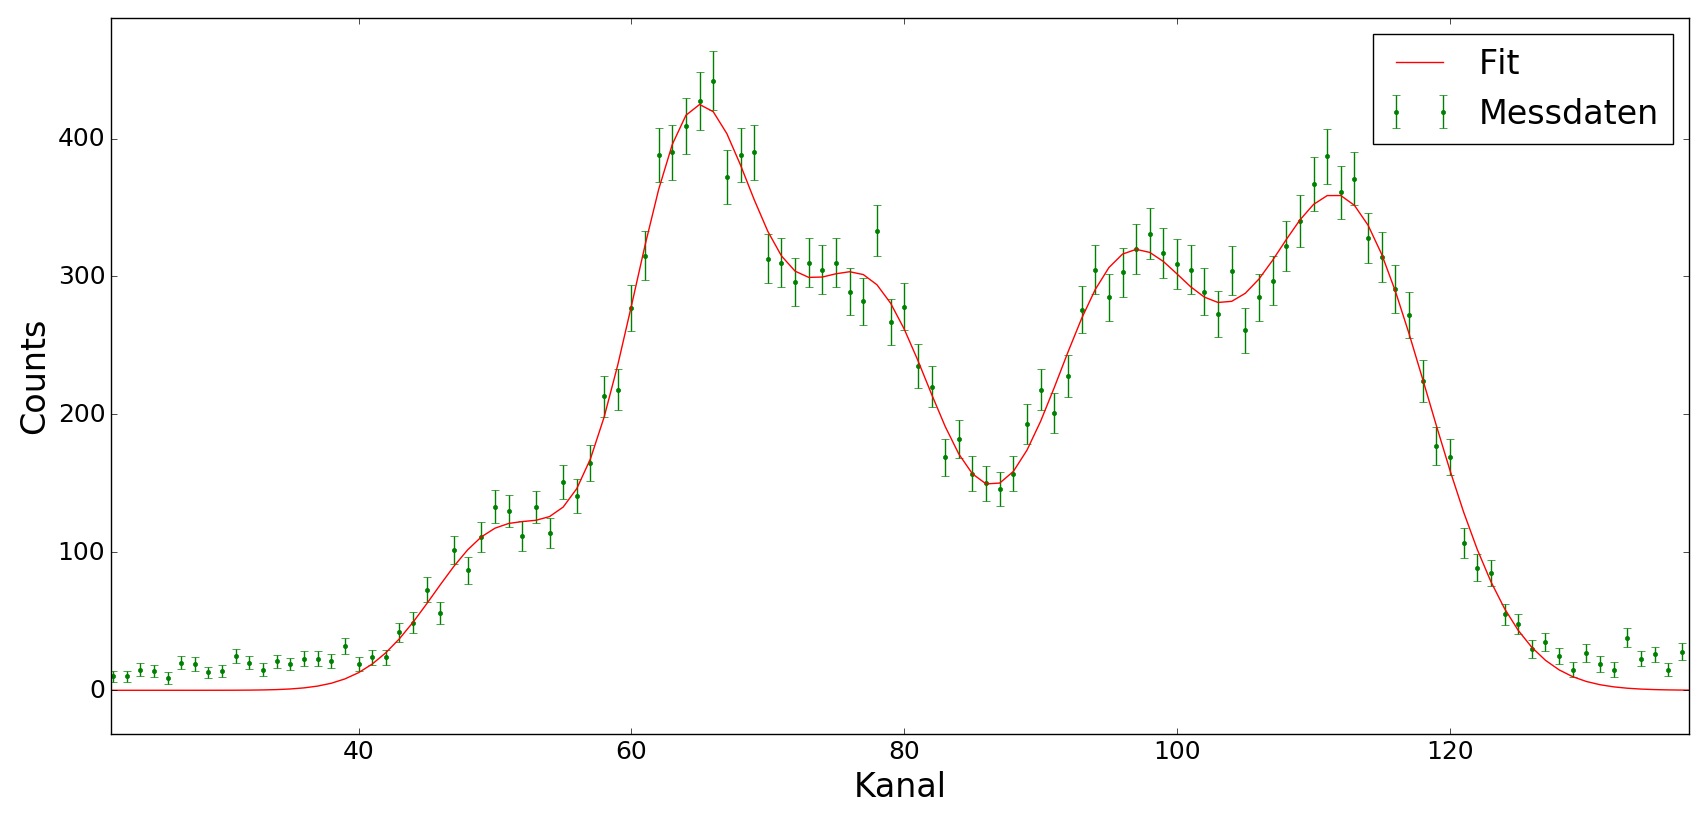
\includegraphics[scale = 0.39]{kalib_fit_1.png}
\caption{Fit der vorderen Peaks f�r $^{241}$Am. Die Fitparameter sind in Tabelle \ref{tab:kalib_fit_1} eingetragen.}
\label{fig:kilb_fit_1}
\end{figure}

\begin{table}[H]
\centering
\caption{Fitparameter f�r die vorderen Peaks der $^{241}$Am Quelle. Das $\chi^2_{red}$ ergab sich mit 1,15}
\label{tab:kalib_fit_1}
\begin{tabular}{|c|c|c|}
\hline Gau�peak & Parameter & Wert \\ 
\hline 1 & Amplitude & 1422(173) \\ 
\hline  & Center & 50,5(7) \\ 
\hline  & Sigma & 5,0(4) \\ 
\hline 2 & Amplitude & 4871(649) \\ 
\hline  & Center & 64,5(5) \\ 
\hline  & Sigma & 4,8(4) \\ 
\hline 3 & Amplitude & 3939(652) \\ 
\hline  & Center & 77,3(7) \\ 
\hline  & Sigma & 5,5(7) \\ 
\hline 4 & Amplitude & 4451(427) \\ 
\hline  & Center & 96,2(4) \\ 
\hline  & Sigma & 5,9(5) \\ 
\hline 5 & Amplitude & 5577(315) \\ 
\hline  & Center & 112,0(4) \\ 
\hline  & Sigma & 6,3(2) \\ 
\hline 
\end{tabular} 
\end{table}


\begin{figure}[H]
\centering
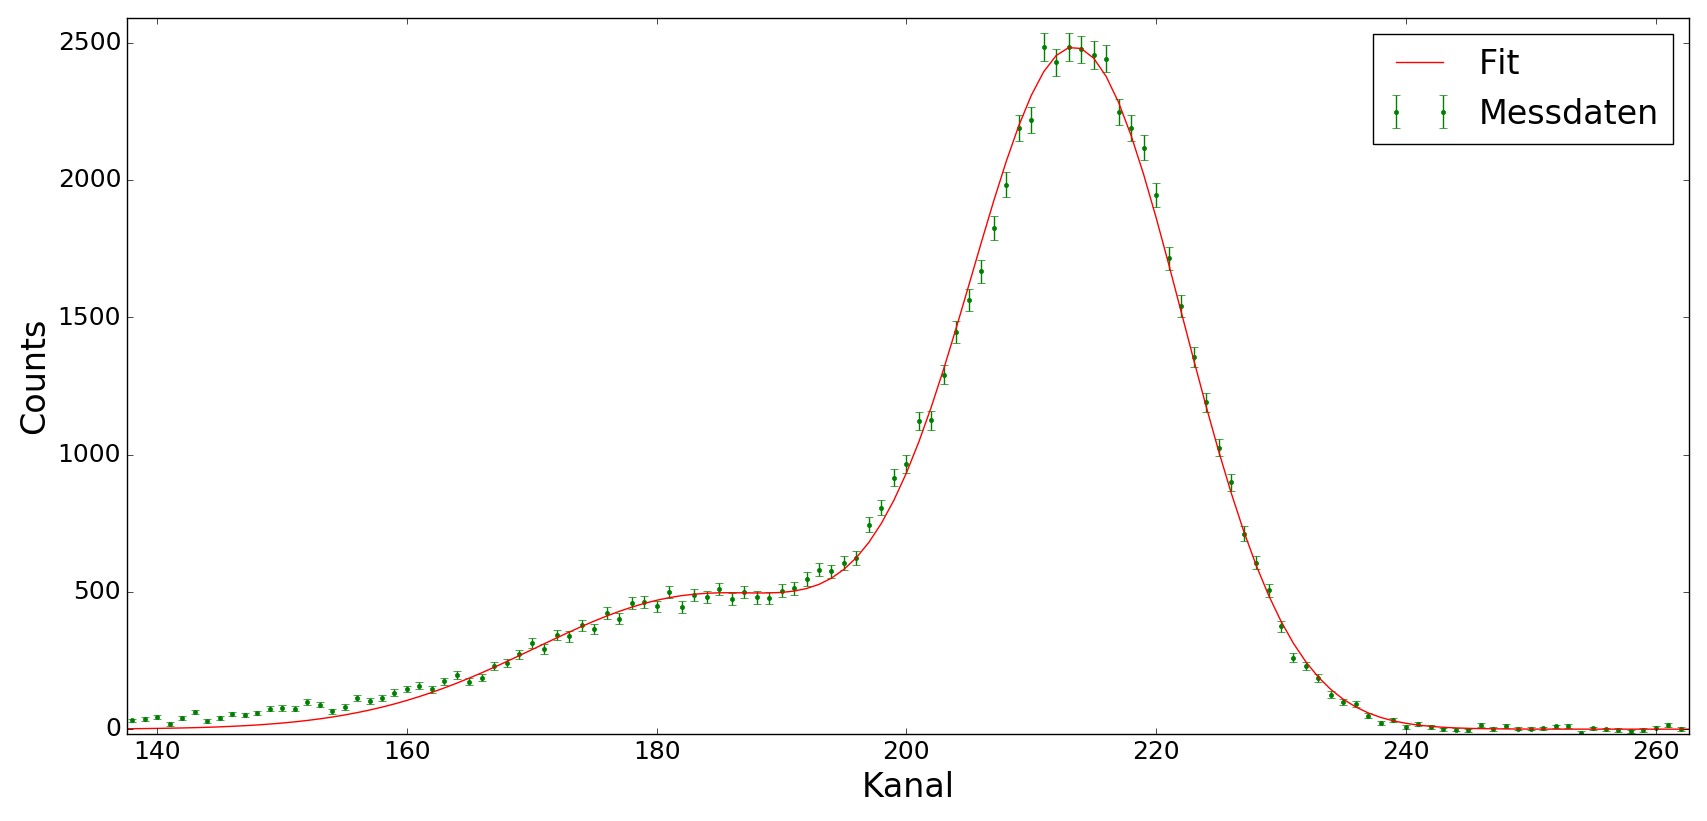
\includegraphics[scale = 0.39]{kalib_fit_2.png}
\caption{Fit des Hauptpeaks f�r $^{241}$Am. Die Fitparameter sind in Tabelle \ref{tab:kalib_fit_2} eingetragen. Das $\chi^2_{red}$ ergab sich mit 1,67}
\label{fig:kalib_fit_2}
\end{figure}

\begin{table}[H]
\centering
\caption{Fitparameter f�r die vorderen Peaks der $^{241}$Am Quelle.}
\label{tab:kalib_fit_2}
\begin{tabular}{|c|c|c|}
\hline Gau�peak & Parameter & Wert \\ 
\hline 1 & Amplitude & 16761(654) \\ 
\hline  & Center & 184(6) \\ 
\hline  & Sigma & 13.7(6) \\ 
\hline 2 & Amplitude & 52316(604) \\ 
\hline  & Center & 213.6(1) \\ 
\hline  & Sigma & 8.56(7) \\ 
\hline 
\end{tabular} 
\end{table}


\begin{figure}[H]
\centering
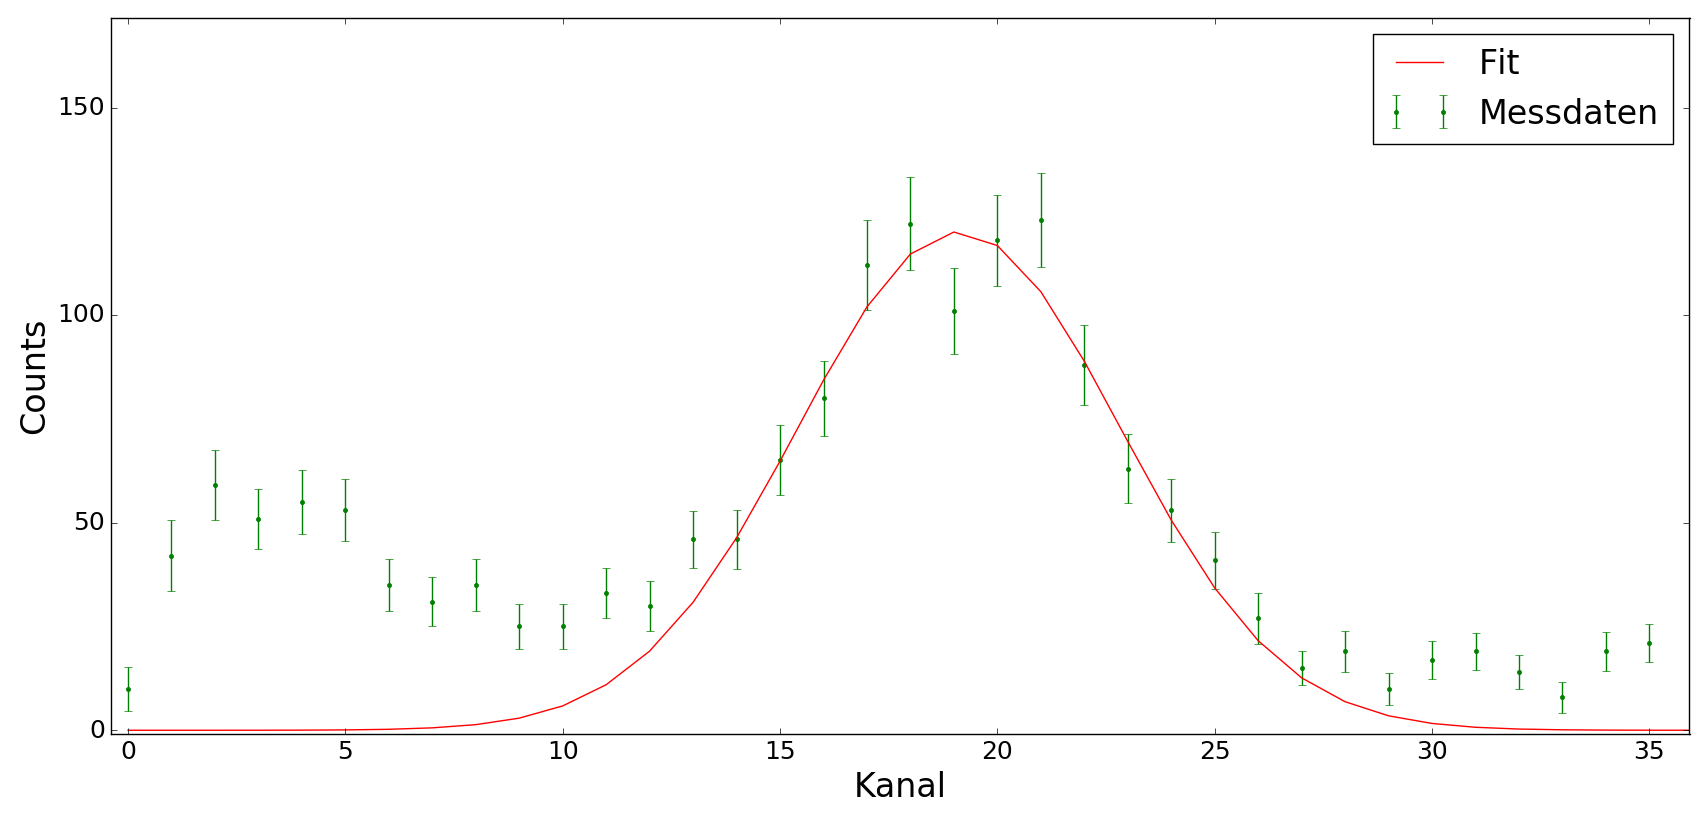
\includegraphics[scale = 0.39]{kalib_fit_3.png}
\caption{Fit des ersten Peaks f�r $^{133}$Ba. Die Fitparameter sind in Tabelle \ref{tab:kalib_fit_3} eingetragen.}
\label{fig:kilb_fit_3}
\end{figure}

\begin{table}[H]
\centering
\caption{Fitparameter f�r die vorderen Peaks der $^{133}$Ba Quelle. Das $\chi^2_{red}$ ergab sich mit 1,14}
\label{tab:kalib_fit_3}
\begin{tabular}{|c|c|c|}
\hline Gau�peak & Parameter & Wert \\ 
\hline 1 & Amplitude & 1118(61) \\ 
\hline  & Center & 19.1(2) \\ 
\hline  & Sigma & 3.7(3) \\ 
\hline 
\end{tabular} 
\end{table}


\begin{figure}[H]
\centering
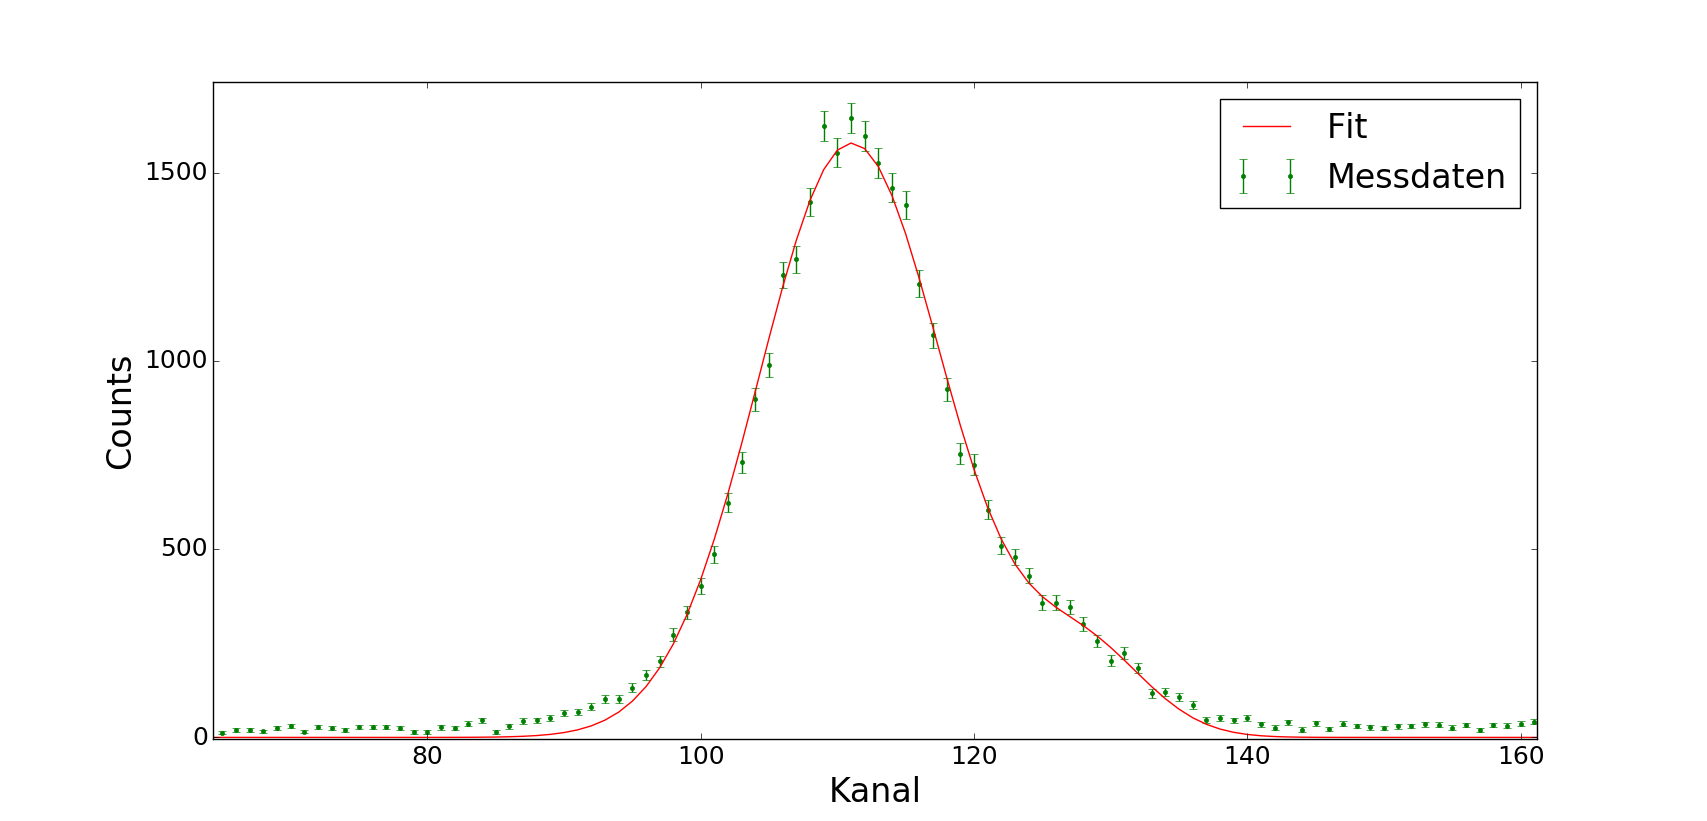
\includegraphics[scale = 0.39]{kalib_fit_4.png}
\caption{Fit des zweiten Peaks f�r $^{133}$Ba. Die Fitparameter sind in Tabelle \ref{tab:kalib_fit_4} eingetragen.}
\label{fig:kilb_fit_4}
\end{figure}

\begin{table}[H]
\centering
\caption{Fitparameter f�r den zweiten Peak der $^{133}$Ba Quelle. Das $\chi^2_{red}$ ergab sich mit 2.31}
\label{tab:kalib_fit_4}
\begin{tabular}{|c|c|c|}
\hline Gau�peak & Parameter & Wert \\ 
\hline 1 & Amplitude & 26864(382) \\ 
\hline  & Center & 111.1(1) \\ 
\hline  & Sigma & 6.8(1) \\ 
\hline 2 & Amplitude & 2615(323) \\ 
\hline  & Center & 128(5) \\ 
\hline  & Sigma & 4.5(5) \\ 
\hline 
\end{tabular} 
\end{table}



\begin{figure}[H]
\centering
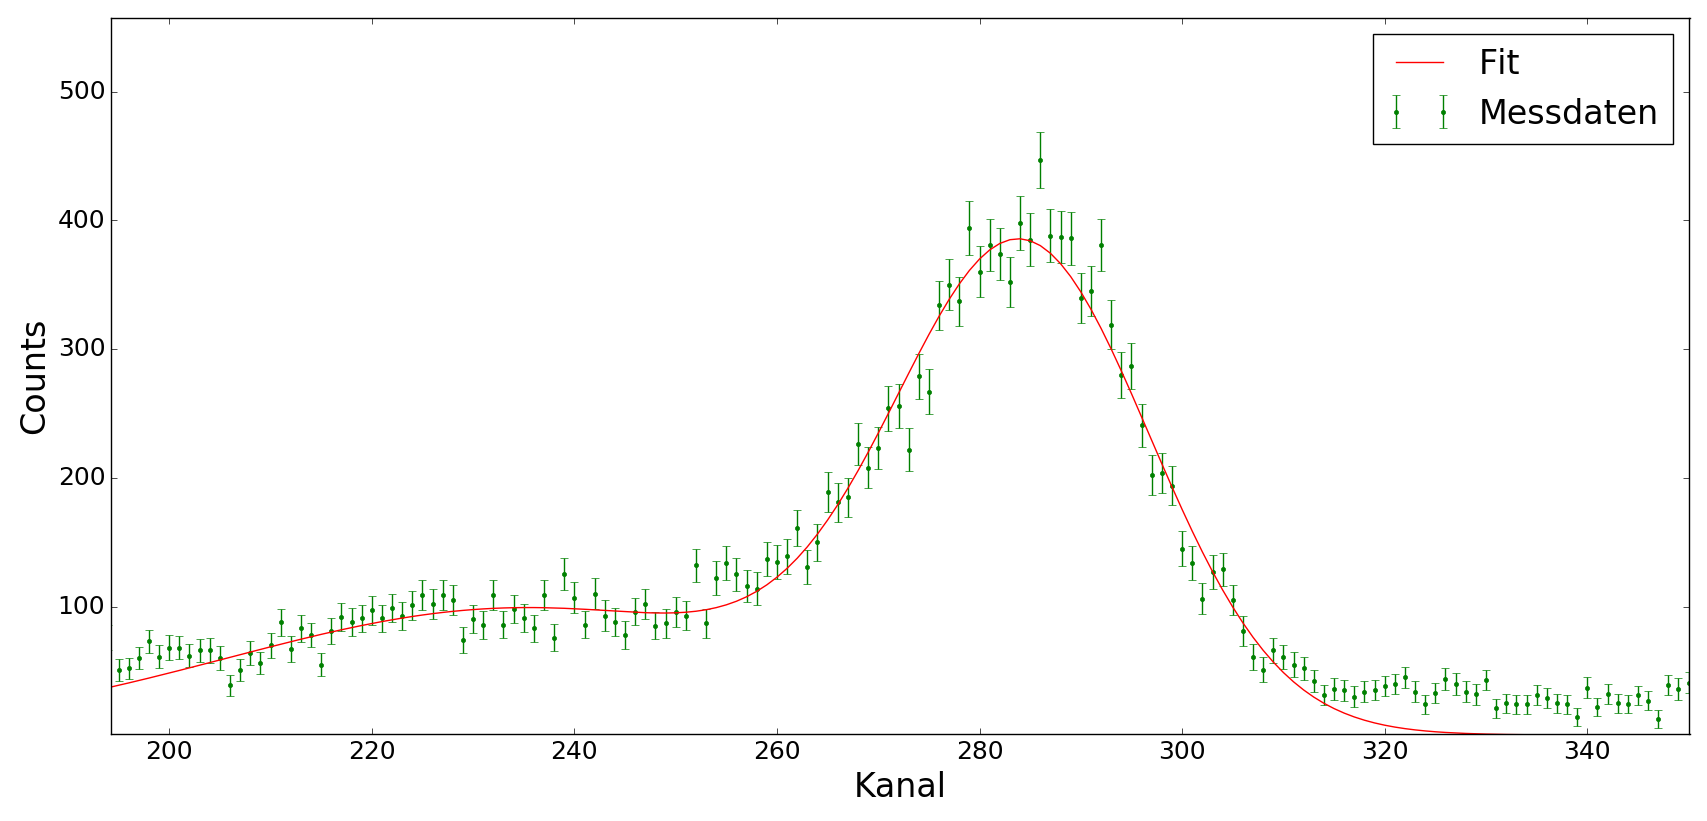
\includegraphics[scale = 0.39]{kalib_fit_5.png}
\caption{Fit des dritten Peaks f�r $^{133}$Ba. Die Fitparameter sind in Tabelle \ref{tab:kalib_fit_5} eingetragen.}
\label{fig:kilb_fit_5}
\end{figure}

\begin{table}[H]
\centering
\caption{Fitparameter f�r die dritten Peaks der $^{133}$Ba Quelle. Das $\chi^2_{red}$ ergab sich mit 1.77}
\label{tab:kalib_fit_5}
\begin{tabular}{|c|c|c|}
\hline Gau�peak & Parameter & Wert \\ 
\hline 1 & Amplitude & 7263(781) \\ 
\hline  & Center & 235(5) \\ 
\hline  & Sigma & 29(4) \\ 
\hline 2 & Amplitude & 11357(560) \\ 
\hline  & Center & 284.4(3) \\ 
\hline  & Sigma & 12.5(3) \\ 
\hline 
\end{tabular} 
\end{table}



\begin{figure}[H]
\centering
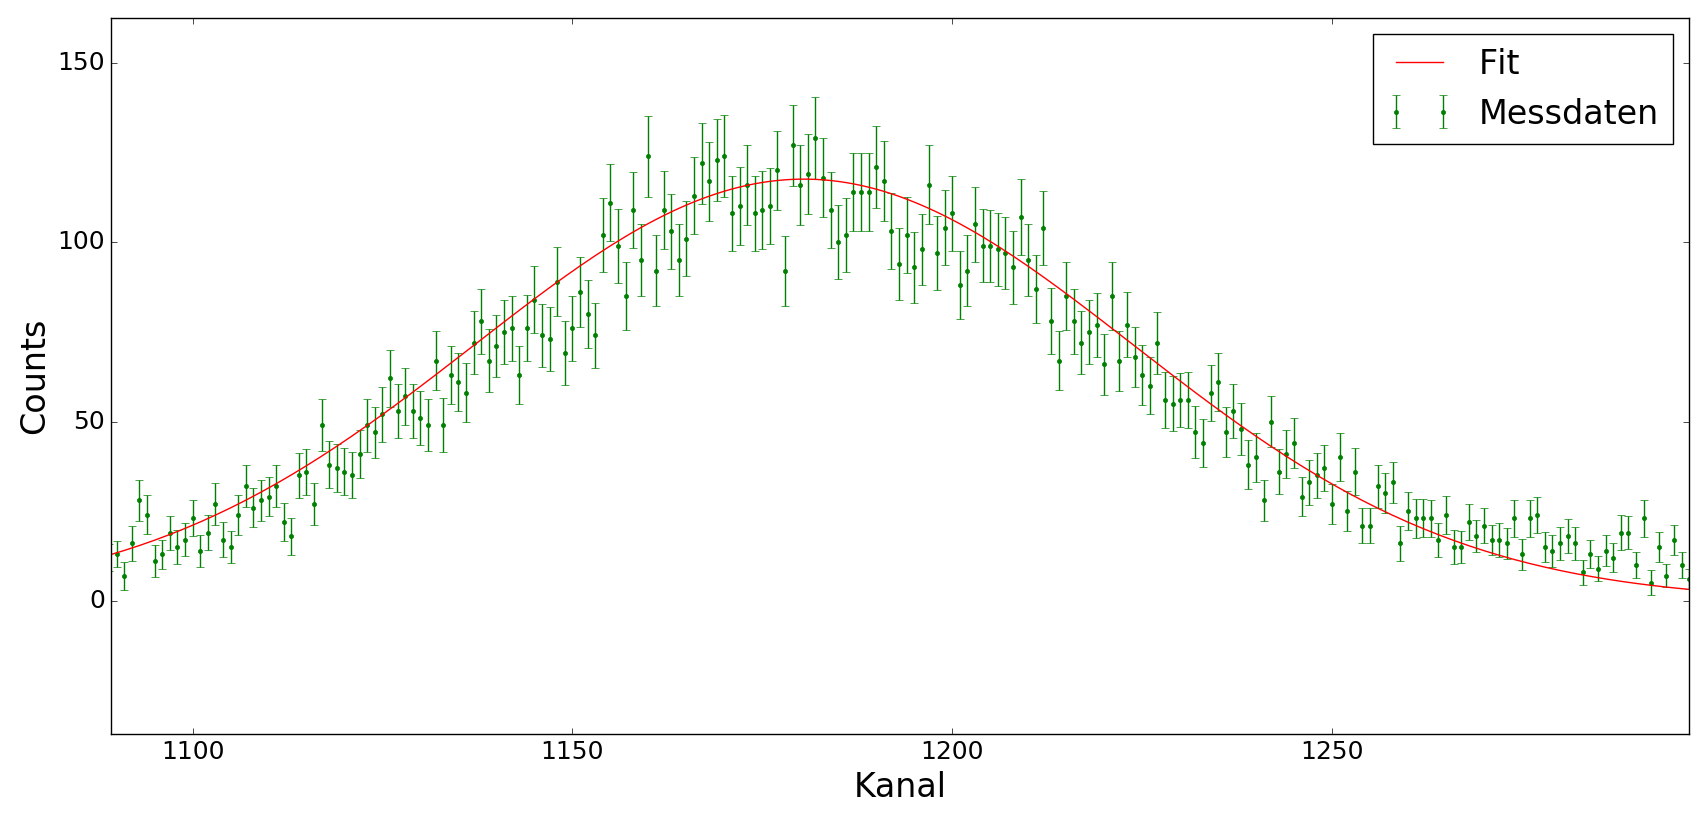
\includegraphics[scale = 0.39]{kalib_fit_6.png}
\caption{Fit des vierten Peaks f�r $^{133}$Ba. Die Fitparameter sind in Tabelle \ref{tab:kalib_fit_6} eingetragen.}
\label{fig:kilb_fit_6}
\end{figure}

\begin{table}[H]
\centering
\caption{Fitparameter des vierten Peaks der $^{133}$Ba Quelle. Das $\chi^2_{red}$ ergab sich mit 0,80}
\label{tab:kalib_fit_6}
\begin{tabular}{|c|c|c|}
\hline Gau�peak & Parameter & Wert \\ 
\hline 1 & Amplitude & 12789(117) \\ 
\hline  & Center & 1180,5(5) \\ 
\hline  & Sigma & 43,4(5) \\ 
\hline 
\end{tabular} 
\end{table}


\begin{figure}[H]
\centering
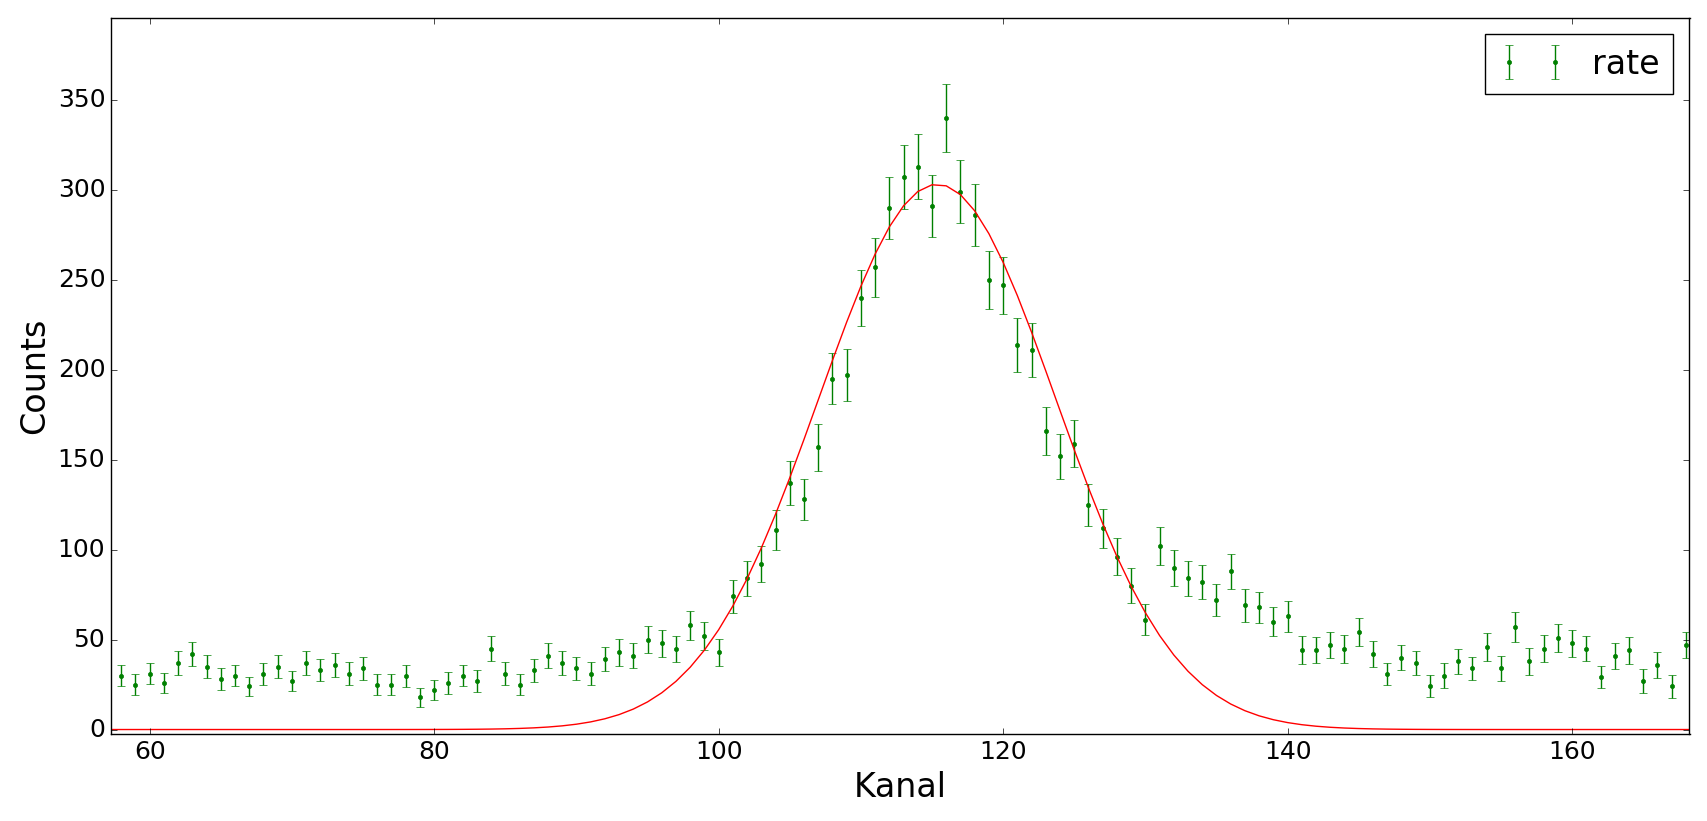
\includegraphics[scale = 0.39]{kalib_fit_7.png}
\caption{Fit des ersten Peaks f�r $^{137}$Cs. Die Fitparameter sind in Tabelle \ref{tab:kalib_fit_7} eingetragen.}
\label{fig:kilb_fit_7}
\end{figure}

\begin{table}[H]
\centering
\caption{Fitparameter des ersten Peaks der $^{137}$Cs Quelle. Das $\chi^2_{red}$ ergab sich mit 1,34}
\label{tab:kalib_fit_7}
\begin{tabular}{|c|c|c|}
\hline Gau�peak & Parameter & Wert \\ 
\hline 1 & Amplitude & 6336(103) \\ 
\hline  & Center & 115,5(2) \\ 
\hline  & Sigma & 8,3(2) \\ 
\hline 
\end{tabular} 
\end{table}

\section{Absorption}
\label{sec:absorption_anhang}

\subsection{Blei}


\begin{figure}[H]
\centering
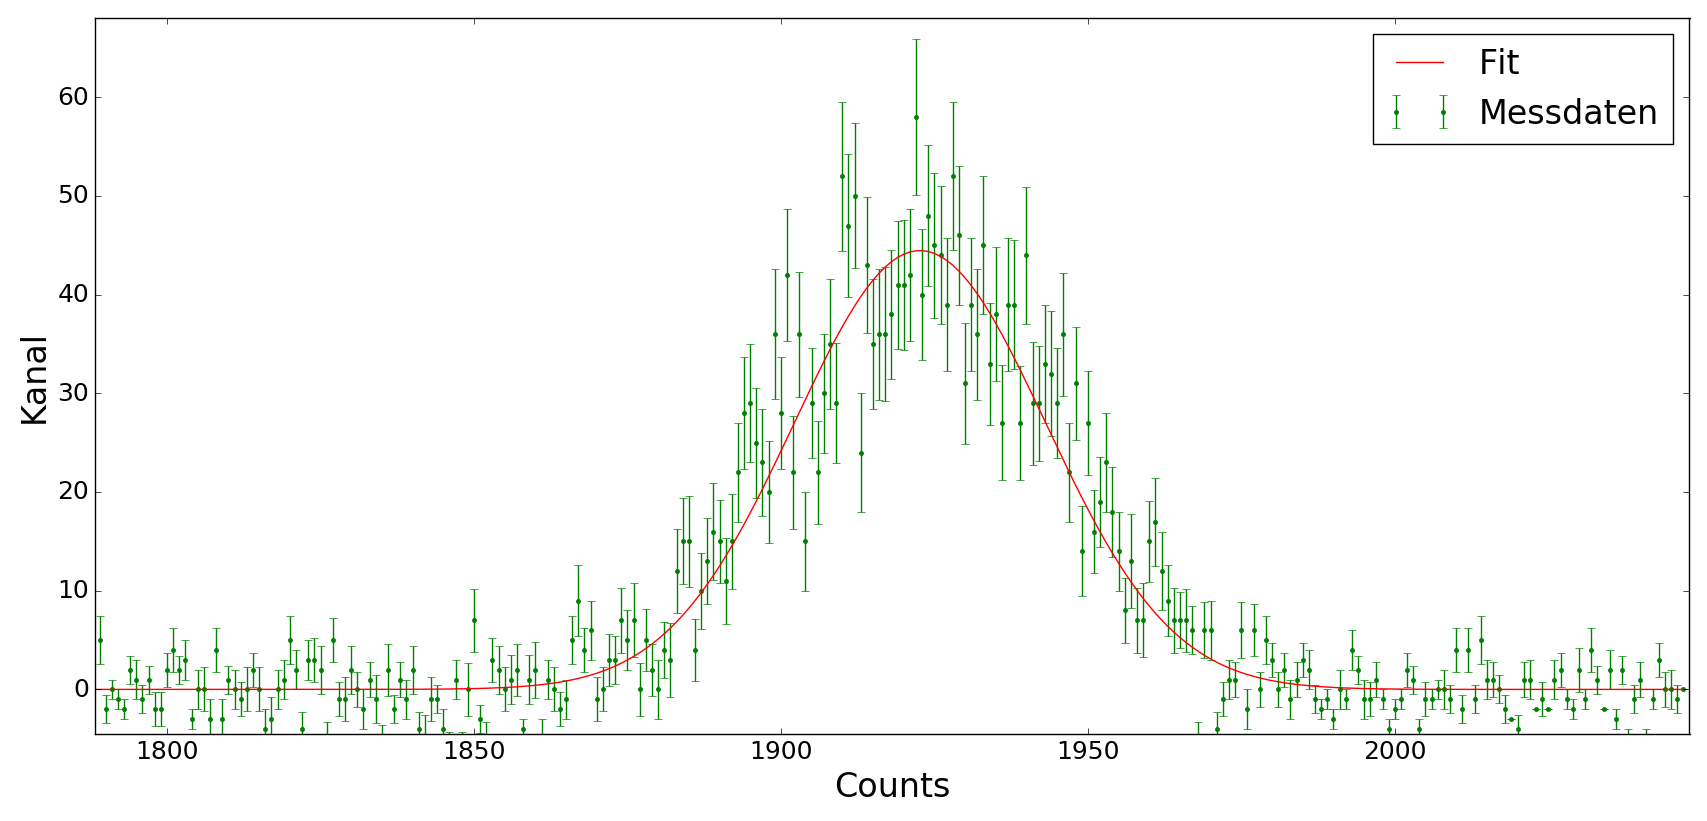
\includegraphics[scale = 0.39]{absrop_fit_blei_1.png}
\caption{Fit des Peaks mit 7,06cm Blei. Die Fitparameter sind in Tabelle \ref{tab:absorp_fit_1} eingetragen.}
\label{fig:absorp_fit_1}
\end{figure}

\begin{table}[H]
\centering
\caption{Fitparameter des Peaks mit 7,06cm Blei. Das $\chi^2_{red}$ ergab sich mit 2,03}
\label{tab:absorp_fit_1}
\begin{tabular}{|c|c|c|}
\hline Gau�peak & Parameter & Wert \\ 
\hline 1 & Amplitude & 2284(77) \\ 
\hline  & Center & 1922,7(7) \\ 
\hline  & Sigma & 20,5(6) \\ 
\hline 
\end{tabular} 
\end{table}


\begin{figure}[H]
\centering
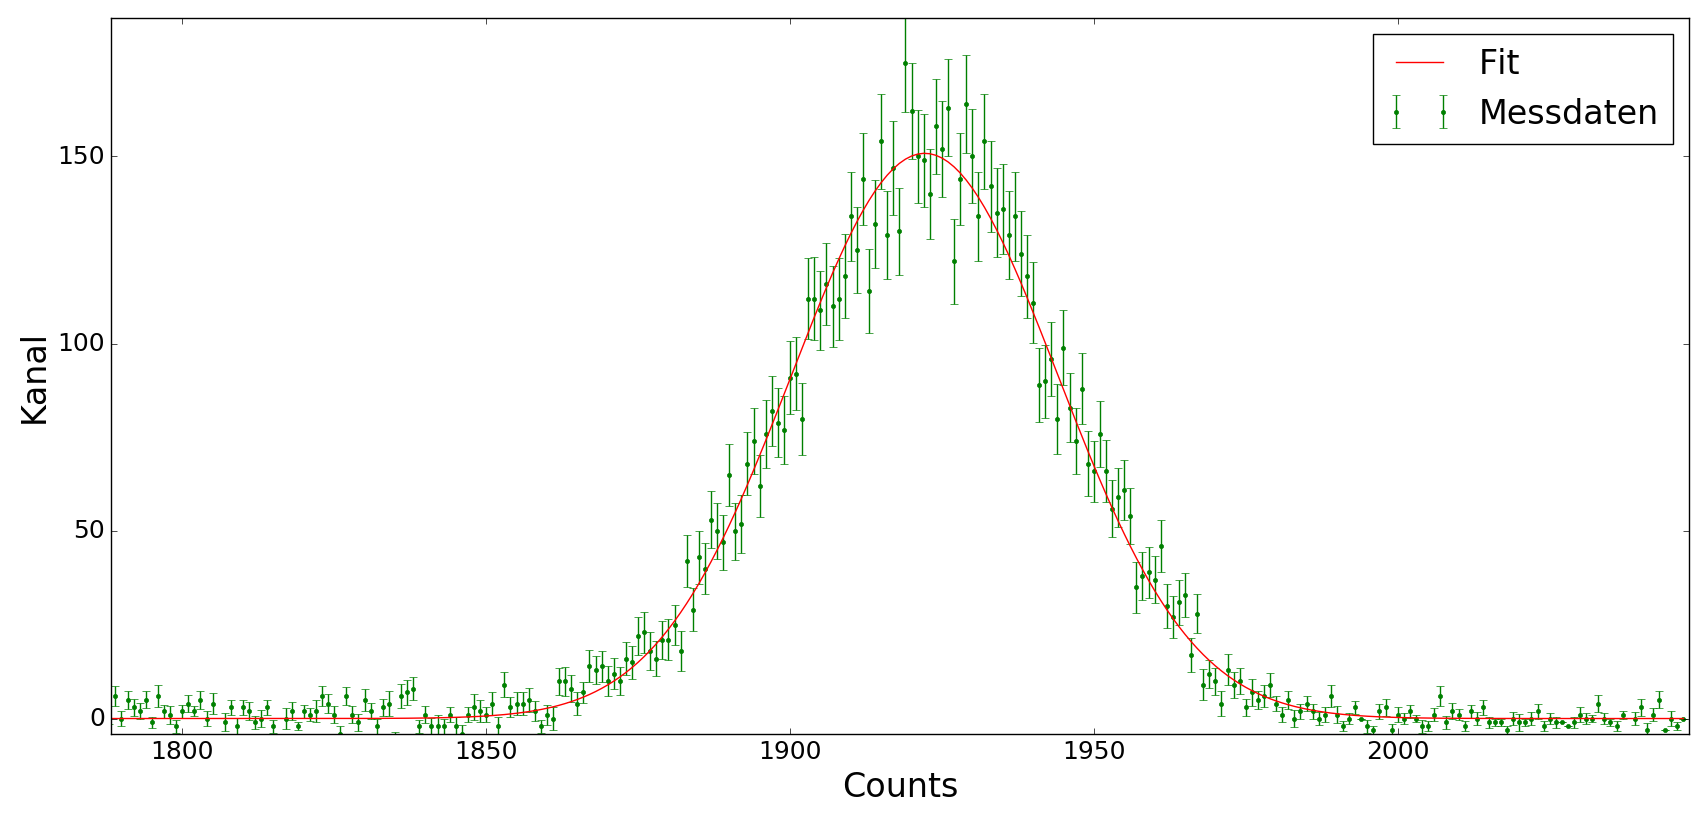
\includegraphics[scale = 0.39]{absrop_fit_blei_2.png}
\caption{Fit des Peaks mit 6,03cm Blei. Die Fitparameter sind in Tabelle \ref{tab:absorp_fit_2} eingetragen.}
\label{fig:absorp_fit_2}
\end{figure}

\begin{table}[H]
\centering
\caption{Fitparameter des Peaks mit 6,03cm Blei. Das $\chi^2_{red}$ ergab sich mit 1,15}
\label{tab:absorp_fit_2}
\begin{tabular}{|c|c|c|}
\hline Gau�peak & Parameter & Wert \\ 
\hline 1 & Amplitude & 8299(101) \\ 
\hline  & Center & 1922,2(3) \\ 
\hline  & Sigma & 22,0(2) \\ 
\hline 
\end{tabular} 
\end{table}



\begin{figure}[H]
\centering
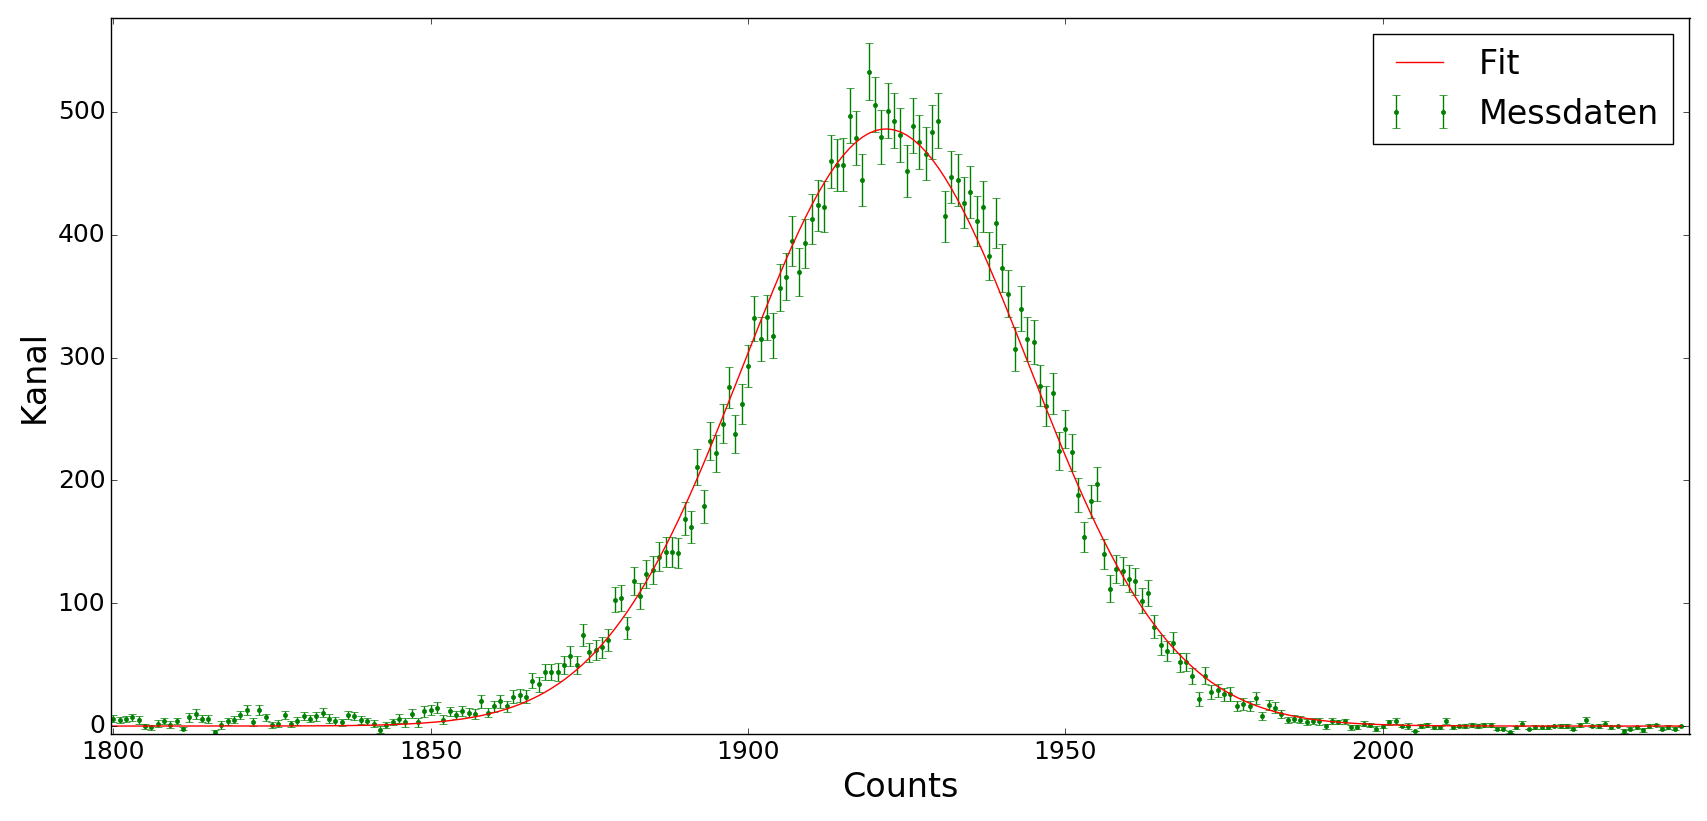
\includegraphics[scale = 0.39]{absrop_fit_blei_3.png}
\caption{Fit des Peaks mit 5,03cm Blei. Die Fitparameter sind in Tabelle \ref{tab:absorp_fit_3} eingetragen.}
\label{fig:absorp_fit_3}
\end{figure}

\begin{table}[H]
\centering
\caption{Fitparameter des Peaks mit 5,03cm Blei. Das $\chi^2_{red}$ ergab sich mit 1,71}
\label{tab:absorp_fit_3}
\begin{tabular}{|c|c|c|}
\hline Gau�peak & Parameter & Wert \\ 
\hline 1 & Amplitude & 27339(220) \\ 
\hline  & Center & 1921,7(2) \\ 
\hline  & Sigma & 22,4(1) \\ 
\hline 
\end{tabular} 
\end{table}



\begin{figure}[H]
\centering
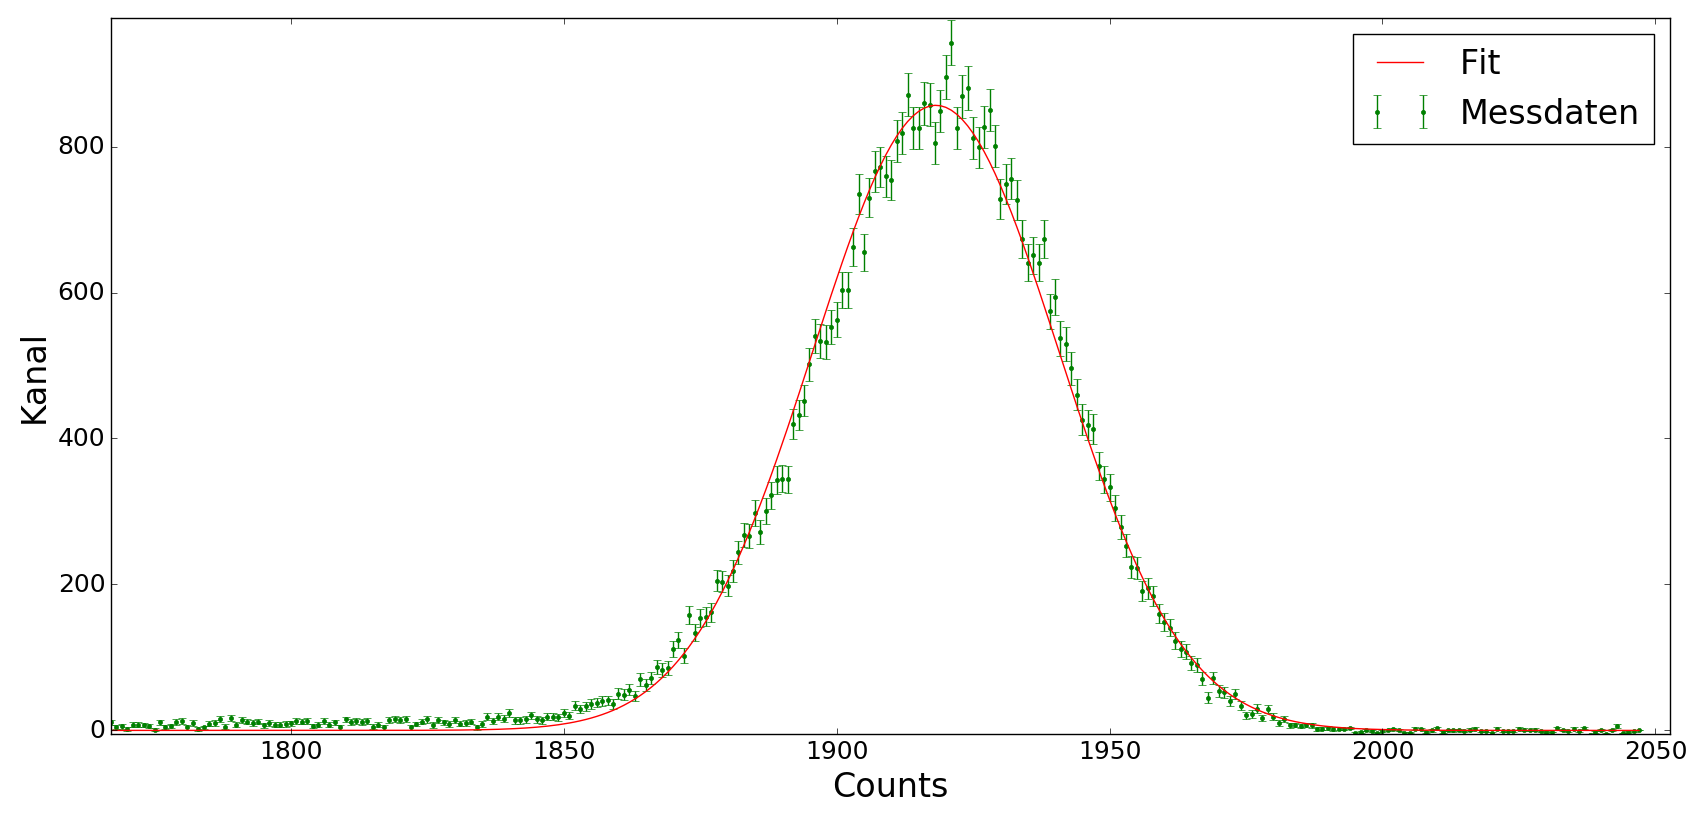
\includegraphics[scale = 0.39]{absrop_fit_blei_4.png}
\caption{Fit des Peaks mit 4,52cm Blei. Die Fitparameter sind in Tabelle \ref{tab:absorp_fit_4} eingetragen.}
\label{fig:absorp_fit_4}
\end{figure}

\begin{table}[H]
\centering
\caption{Fitparameter des Peaks mit 4,52cm Blei. Das $\chi^2_{red}$ ergab sich mit 2,52}
\label{tab:absorp_fit_4}
\begin{tabular}{|c|c|c|}
\hline Gau�peak & Parameter & Wert \\ 
\hline 1 & Amplitude & 48414(352) \\ 
\hline  & Center & 1918,2(2) \\ 
\hline  & Sigma & 22,6(1) \\ 
\hline 
\end{tabular} 
\end{table}



\begin{figure}[H]
\centering
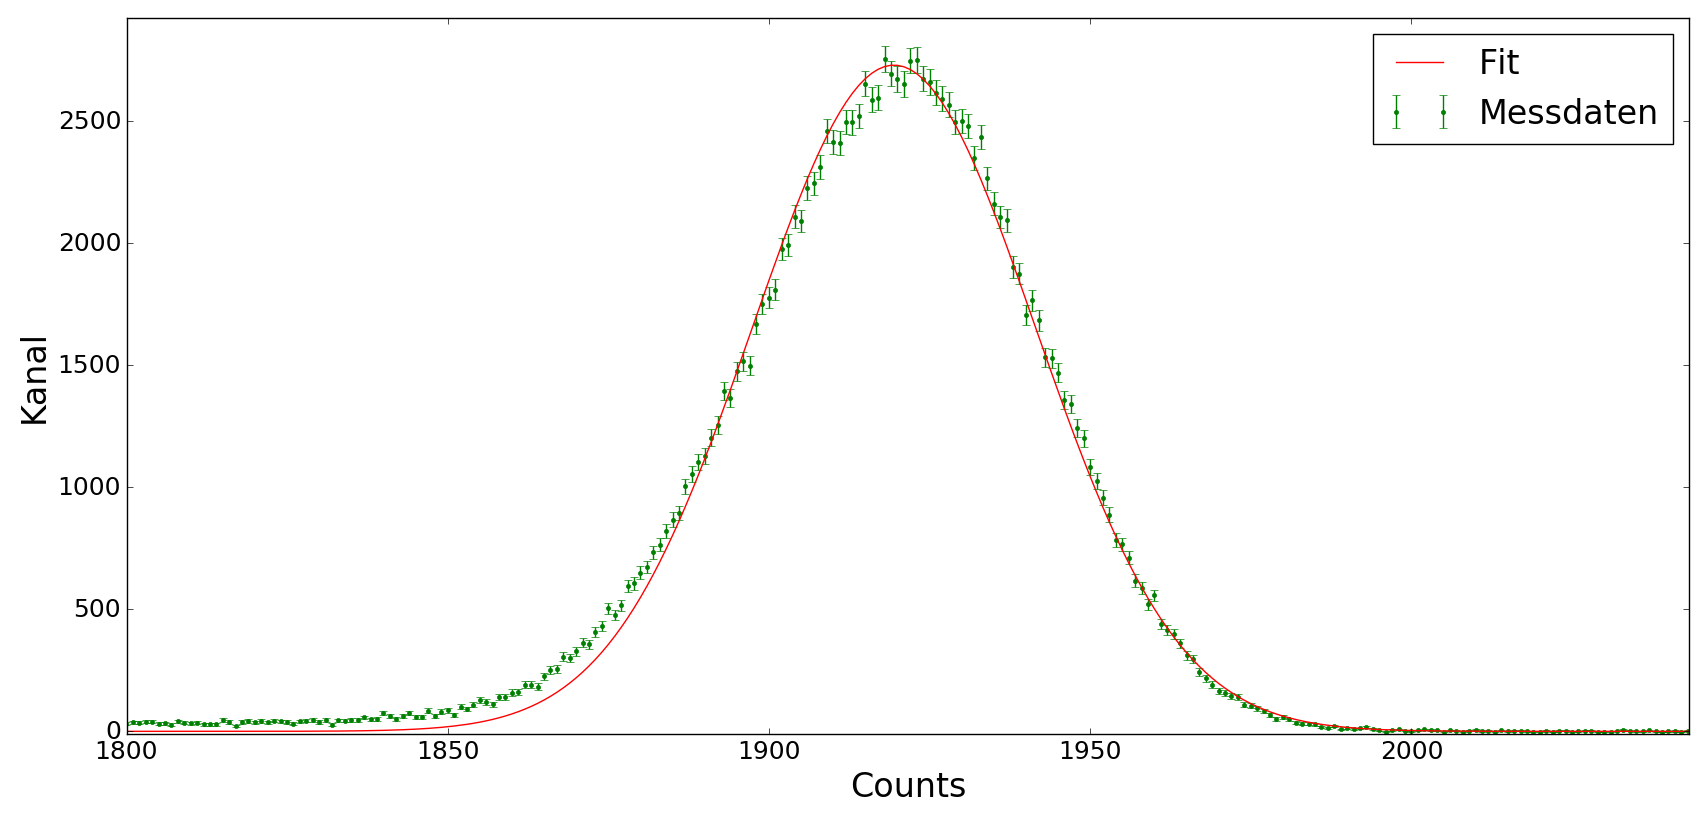
\includegraphics[scale = 0.39]{absrop_fit_blei_5.png}
\caption{Fit des Peaks mit 3,51cm Blei. Die Fitparameter sind in Tabelle \ref{tab:absorp_fit_5} eingetragen.}
\label{fig:absorp_fit_5}
\end{figure}

\begin{table}[H]
\centering
\caption{Fitparameter des Peaks mit 3,51cm Blei. Das $\chi^2_{red}$ ergab sich mit 2,72}
\label{tab:absorp_fit_5}
\begin{tabular}{|c|c|c|}
\hline Gau�peak & Parameter & Wert \\ 
\hline 1 & Amplitude & 150770(666) \\ 
\hline  & Center & 1919,5(1) \\ 
\hline  & Sigma & 22,02(9) \\ 
\hline 
\end{tabular} 
\end{table}





\begin{figure}[H]
\centering
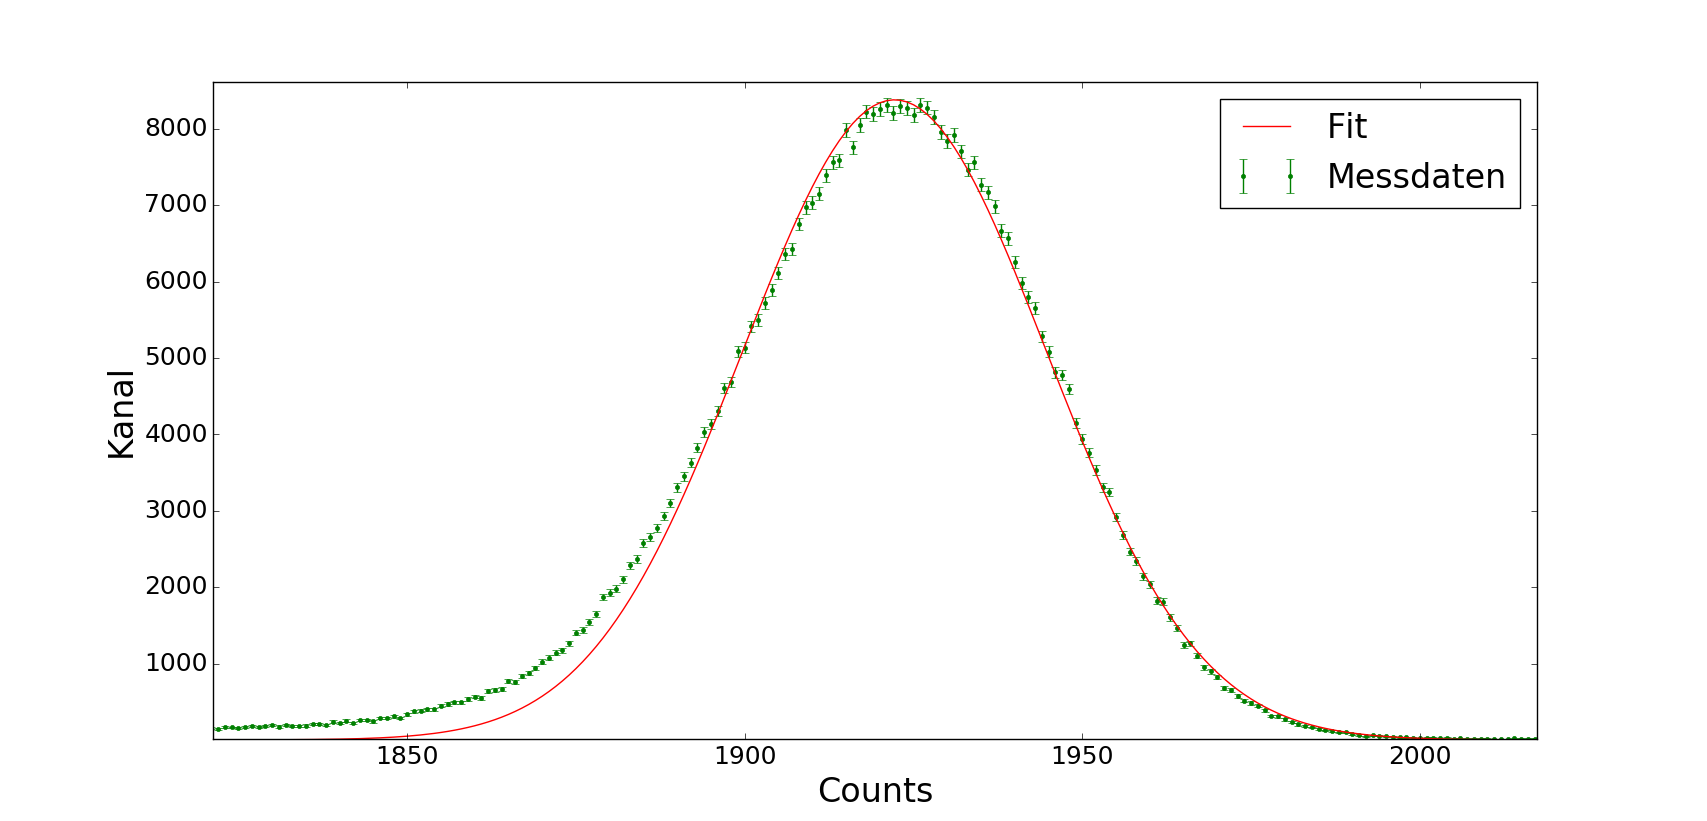
\includegraphics[scale = 0.39]{absrop_fit_blei_6.png}
\caption{Fit des Peaks mit 2,50cm Blei. Die Fitparameter sind in Tabelle \ref{tab:absorp_fit_6} eingetragen.}
\label{fig:absorp_fit_6}
\end{figure}

\begin{table}[H]
\centering
\caption{Fitparameter des Peaks mit 2,50cm Blei. Das $\chi^2_{red}$ ergab sich mit 4,18}
\label{tab:absorp_fit_6}
\begin{tabular}{|c|c|c|}
\hline Gau�peak & Parameter & Wert \\ 
\hline 1 & Amplitude & 473140(1630) \\ 
\hline  & Center & 1922,18(9) \\ 
\hline  & Sigma & 22,52(9) \\ 
\hline 
\end{tabular} 
\end{table}


\subsection{Aluminium}

\begin{figure}[H]
\centering
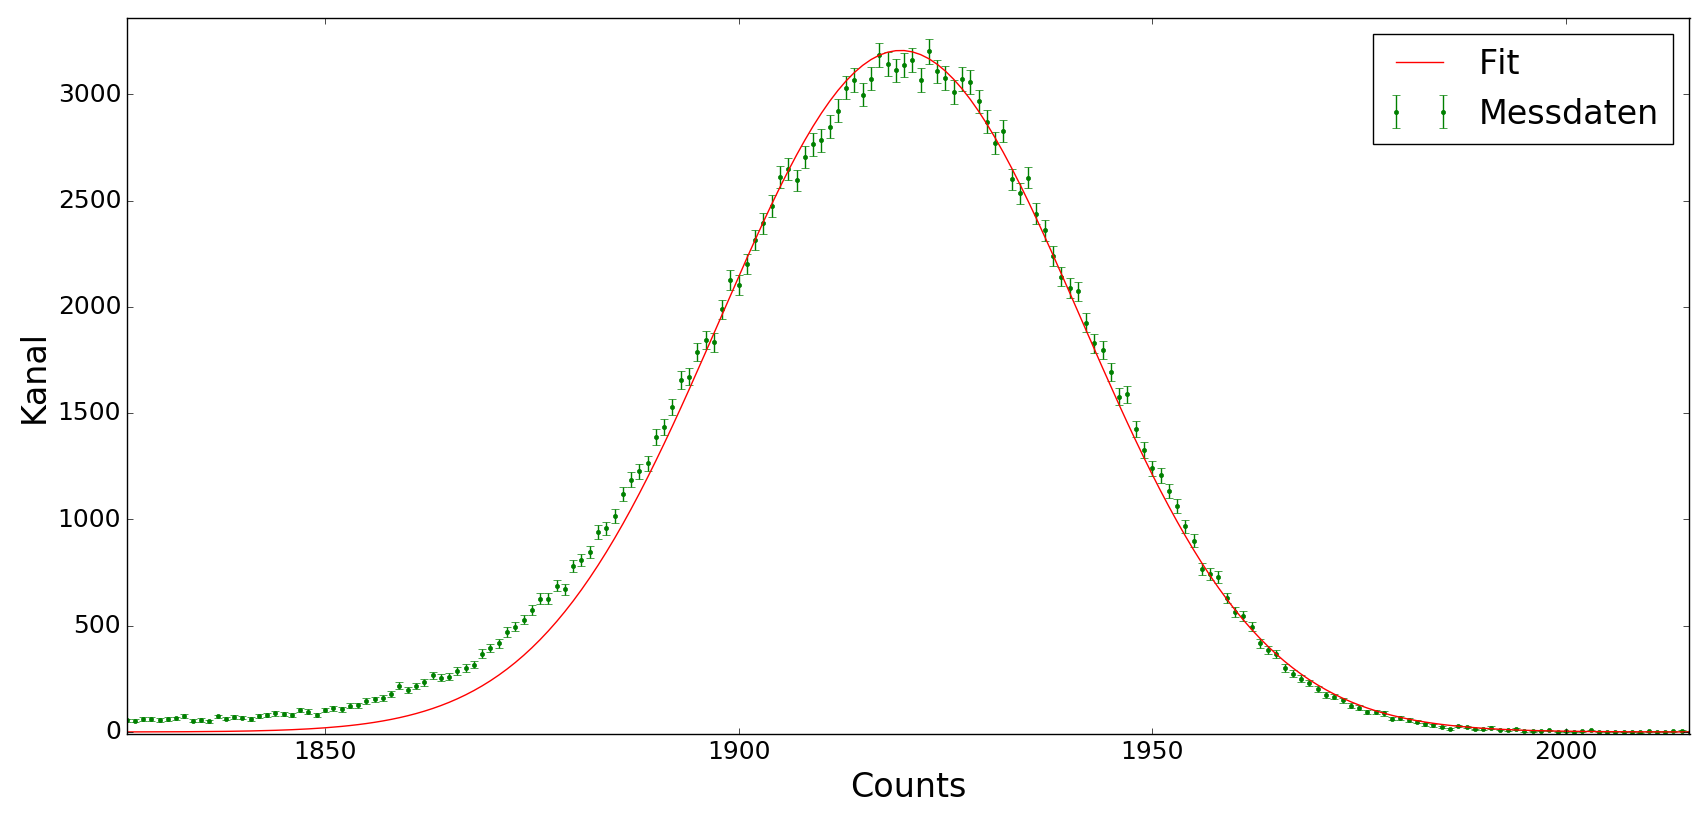
\includegraphics[scale = 0.39]{absrop_fit_alu_1.png}
\caption{Fit des Peaks mit 7,60cm Aluminium. Die Fitparameter sind in Tabelle \ref{tab:absorp_fit_alu_1} eingetragen.}
\label{fig:absorp_fit_alu_1}
\end{figure}

\begin{table}[H]
\centering
\caption{Fitparameter des Peaks mit 7,60cm Blei. Das $\chi^2_{red}$ ergab sich mit 2,18}
\label{tab:absorp_fit_alu_1}
\begin{tabular}{|c|c|c|}
\hline Gau�peak & Parameter & Wert \\ 
\hline 1 & Amplitude & 17520(705) \\ 
\hline  & Center & 1919,5(1) \\ 
\hline  & Sigma & 21,79(8) \\ 
\hline 
\end{tabular} 
\end{table}



\begin{figure}[H]
\centering
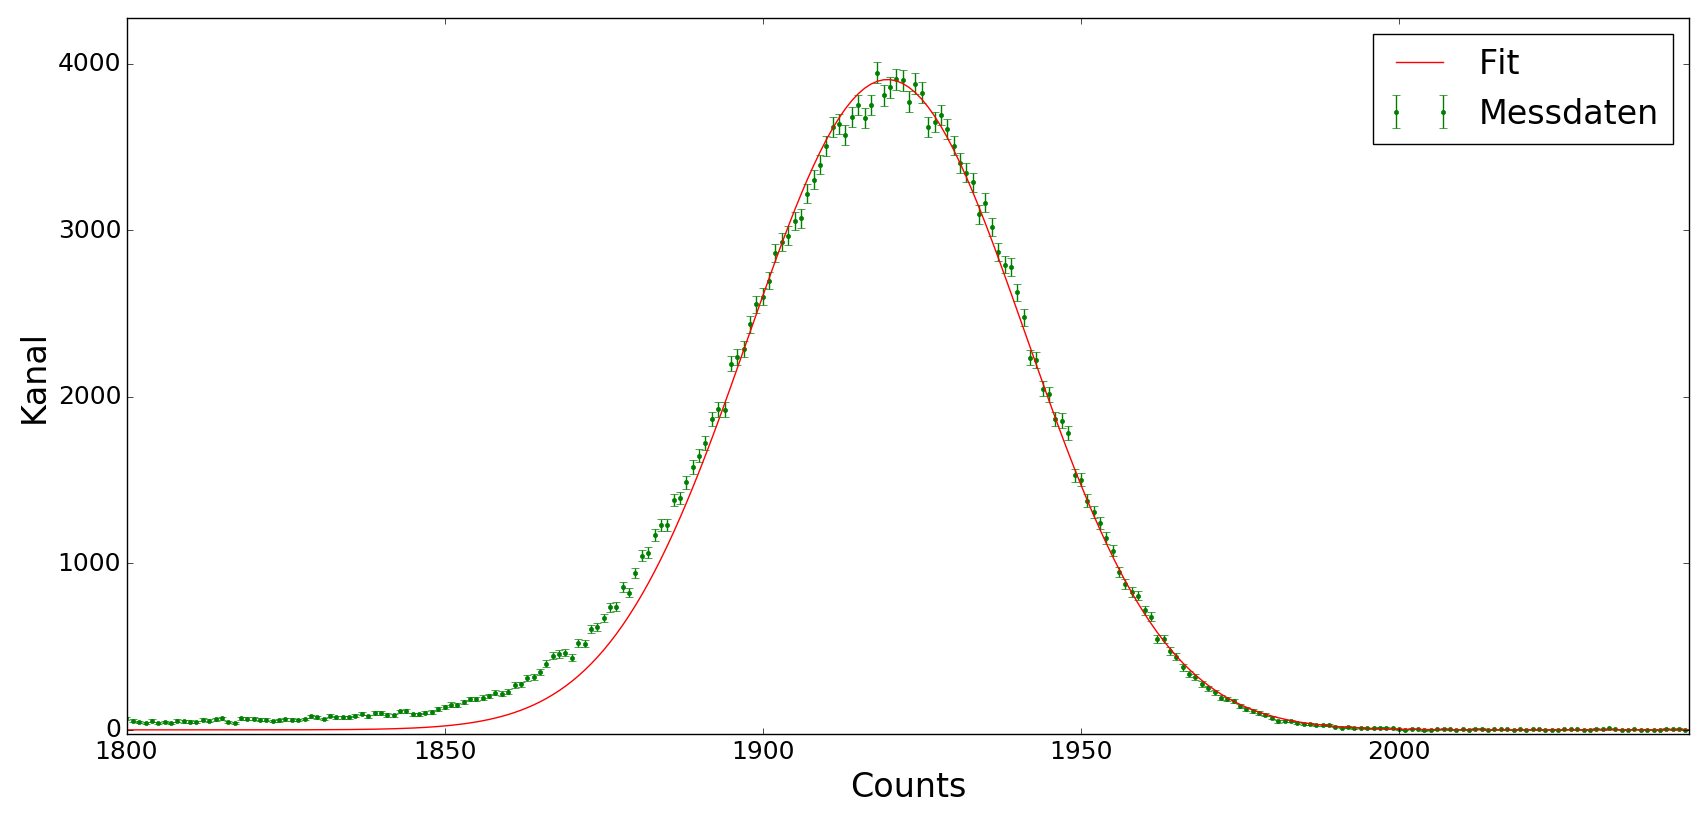
\includegraphics[scale = 0.39]{absrop_fit_alu_2.png}
\caption{Fit des Peaks mit 6,58cm Aluminium. Die Fitparameter sind in Tabelle \ref{tab:absorp_fit_alu_2} eingetragen.}
\label{fig:absorp_fit_alu_2}
\end{figure}

\begin{table}[H]
\centering
\caption{Fitparameter des Peaks mit 6,58cm Blei. Das $\chi^2_{red}$ ergab sich mit 1,77}
\label{tab:absorp_fit_alu_2}
\begin{tabular}{|c|c|c|}
\hline Gau�peak & Parameter & Wert \\ 
\hline 1 & Amplitude & 213170(696) \\ 
\hline  & Center & 1919,59(9) \\ 
\hline  & Sigma & 21,77(7) \\ 
\hline 
\end{tabular} 
\end{table}



\begin{figure}[H]
\centering
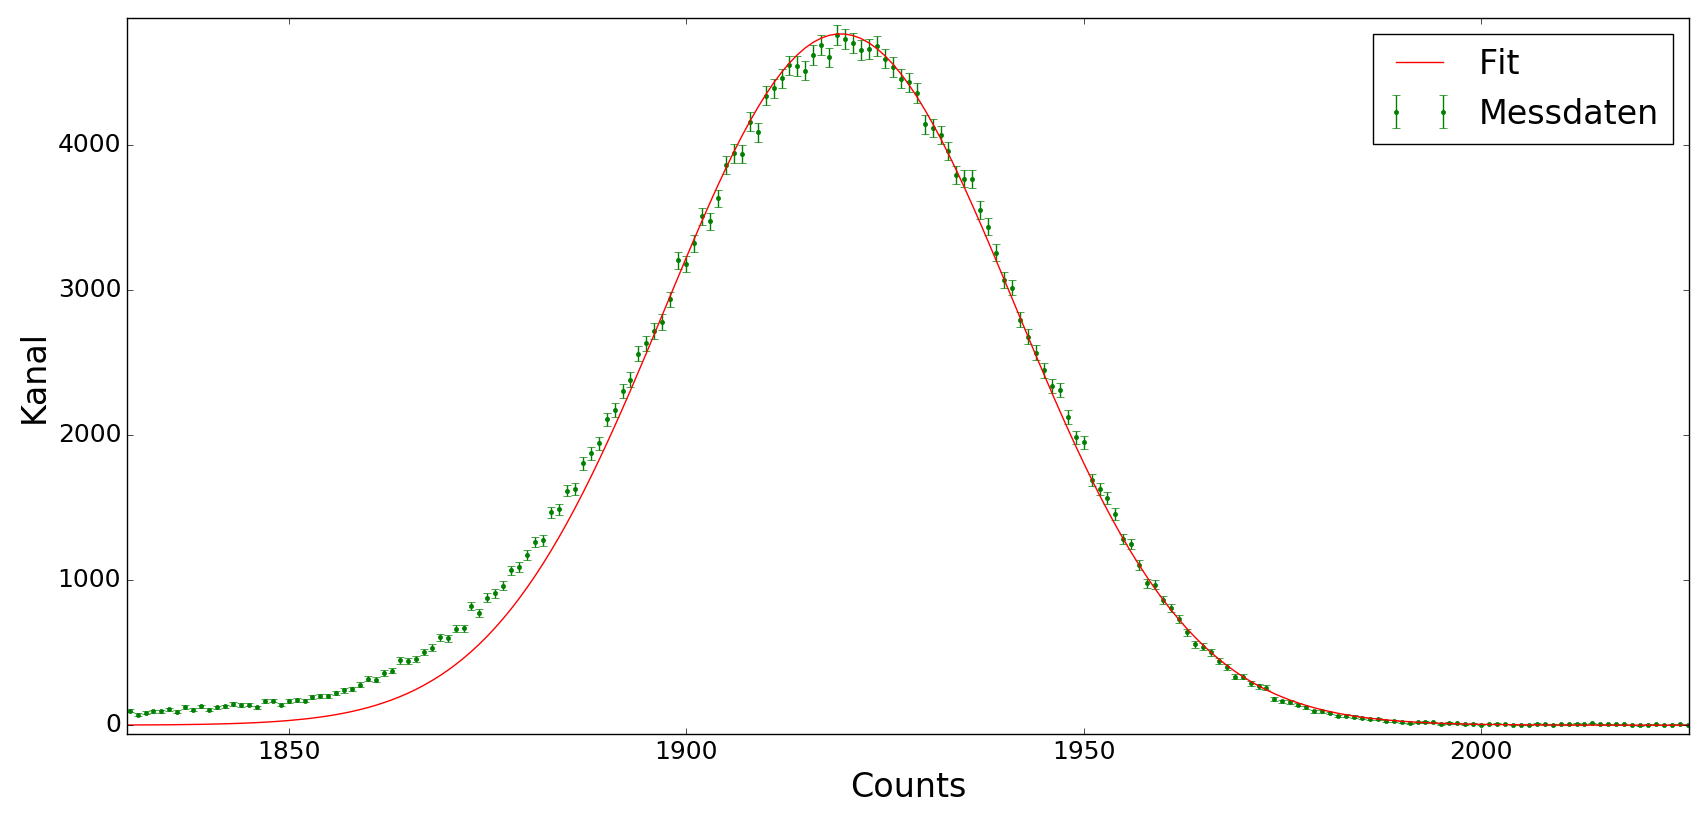
\includegraphics[scale = 0.39]{absrop_fit_alu_3.png}
\caption{Fit des Peaks mit 5,57cm Aluminium. Die Fitparameter sind in Tabelle \ref{tab:absorp_fit_alu_3} eingetragen.}
\label{fig:absorp_fit_alu_3}
\end{figure}

\begin{table}[H]
\centering
\caption{Fitparameter des Peaks mit 5,57cm Blei. Das $\chi^2_{red}$ ergab sich mit 1,91}
\label{tab:absorp_fit_alu_3}
\begin{tabular}{|c|c|c|}
\hline Gau�peak & Parameter & Wert \\ 
\hline 1 & Amplitude & 262160(815) \\ 
\hline  & Center & 1919,43(9) \\ 
\hline  & Sigma & 21,95(7) \\ 
\hline 
\end{tabular} 
\end{table}


\begin{figure}[H]
\centering
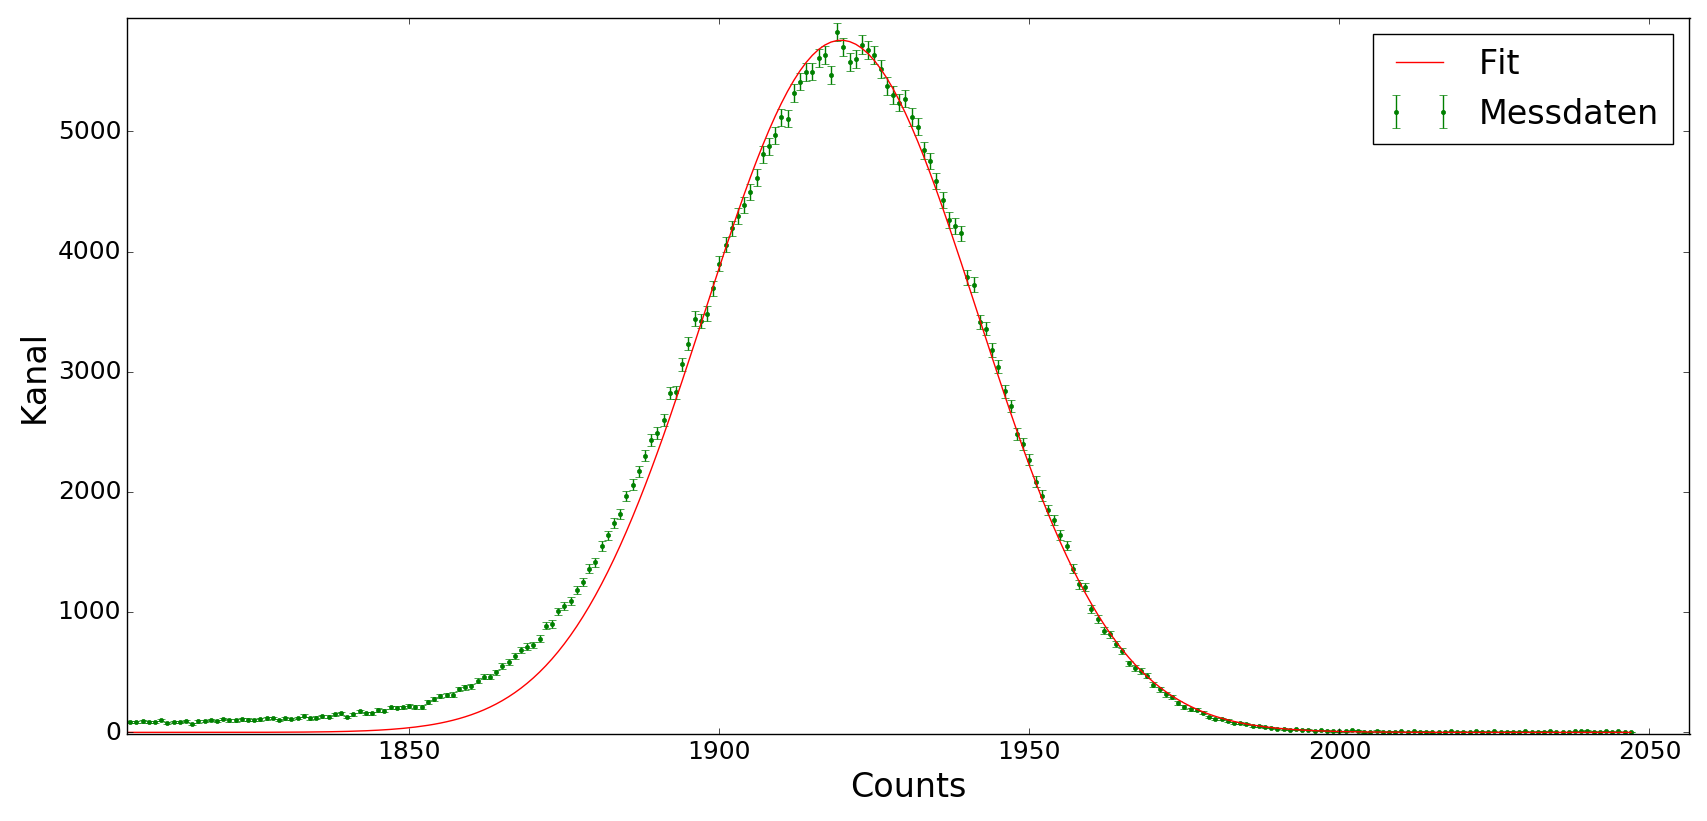
\includegraphics[scale = 0.39]{absrop_fit_alu_4.png}
\caption{Fit des Peaks mit 4,55cm Aluminium. Die Fitparameter sind in Tabelle \ref{tab:absorp_fit_alu_4} eingetragen.}
\label{fig:absorp_fit_alu_4}
\end{figure}

\begin{table}[H]
\centering
\caption{Fitparameter des Peaks mit 4,55cm Blei. Das $\chi^2_{red}$ ergab sich mit 2,32}
\label{tab:absorp_fit_alu_4}
\begin{tabular}{|c|c|c|}
\hline Gau�peak & Parameter & Wert \\ 
\hline 1 & Amplitude & 317600(982) \\ 
\hline  & Center & 1919,62(9) \\ 
\hline  & Sigma & 22,00(7) \\ 
\hline 
\end{tabular} 
\end{table}



\begin{figure}[H]
\centering
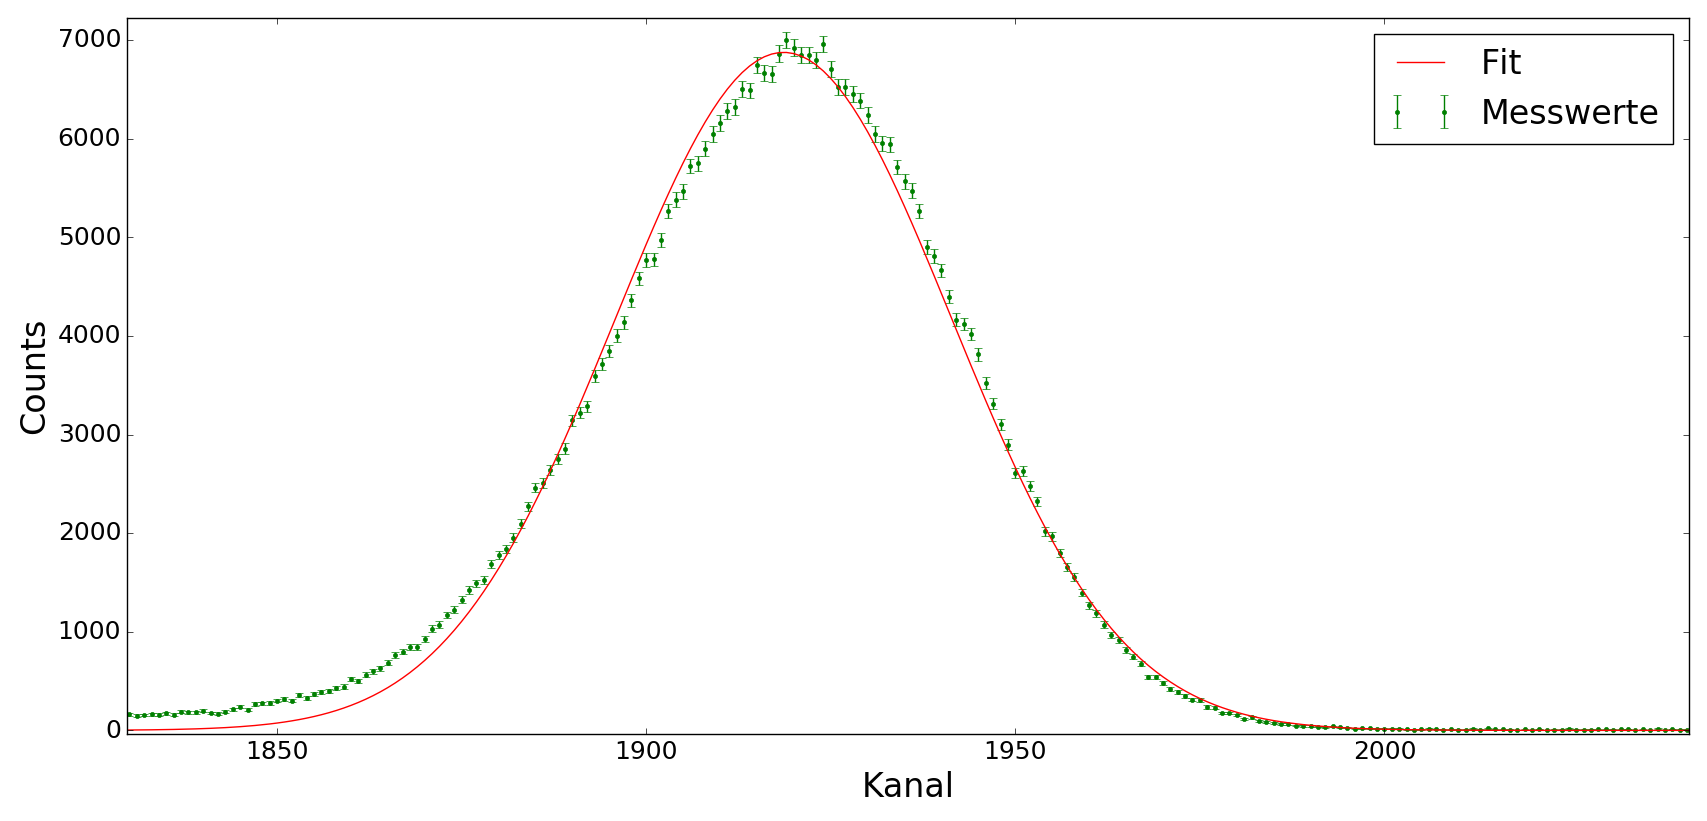
\includegraphics[scale = 0.39]{absrop_fit_alu_5.png}
\caption{Fit des Peaks mit 3,54cm Aluminium. Die Fitparameter sind in Tabelle \ref{tab:absorp_fit_alu_5} eingetragen.}
\label{fig:absorp_fit_alu_5}
\end{figure}

\begin{table}[H]
\centering
\caption{Fitparameter des Peaks mit 3,54cm Blei. Das $\chi^2_{red}$ ergab sich mit 8,72}
\label{tab:absorp_fit_alu_5}
\begin{tabular}{|c|c|c|}
\hline Gau�peak & Parameter & Wert \\ 
\hline 1 & Amplitude & 393100(1880) \\ 
\hline  & Center & 1918,6(1) \\ 
\hline  & Sigma & 22,81(9) \\ 
\hline 
\end{tabular} 
\end{table}
\section{Wirkungsquerschnitt}
In diesem Abschnitt werden die Plots und Fits der Energiemessungen f�r die Winkel von \SI{20}{\degree} bis \SI{80}{\degree} mit den zugeh�rigen Fitparametern dargestellt.
\label{Anh:WQ}
\begin{figure}[H]
\centering
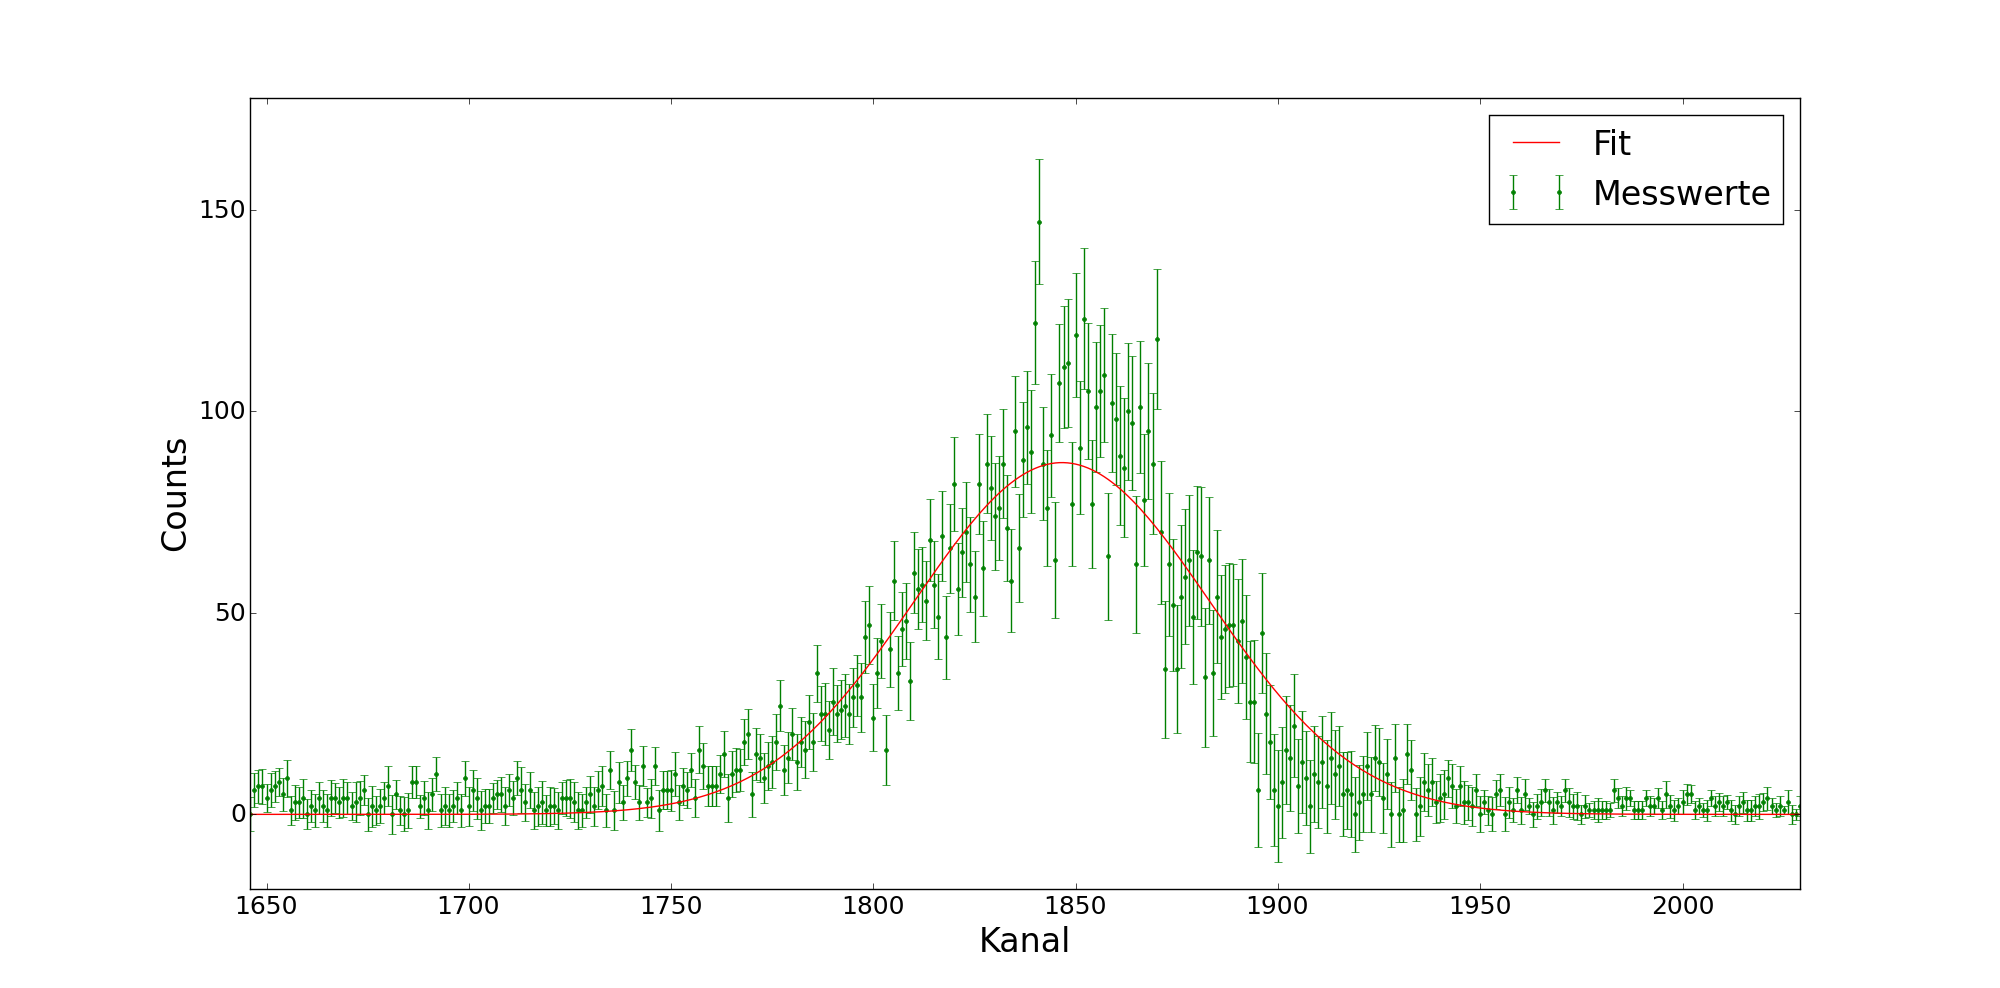
\includegraphics[scale = 0.34]{Wirkungsquerschnitt_20_Grad_Fit.png}
\caption{Die Fitparameter sind in Tabelle \ref{tab:20_Grad_WQ} eingetragen.}
\label{fig:Wirkungsquerschnitt_20}
\end{figure}

\begin{table}[H]
\centering
\caption{Fitparameter f�r die Energiemessung bei \SI{20}{\degree}. Das $\chi^2_{red}$ ergab sich mit 1,099}
\label{tab:20_Grad_WQ}
\begin{tabular}{|c|c|c|}
\hline Gau�peak & Parameter & Wert \\ 
\hline 1 & Amplitude & 8804(270) \\ 
\hline  & Center & 1845.4(7) \\ 
\hline  & Sigma & 34.3(8) \\ 
\hline 
\end{tabular} 
\end{table}

\begin{figure}[H]
\centering
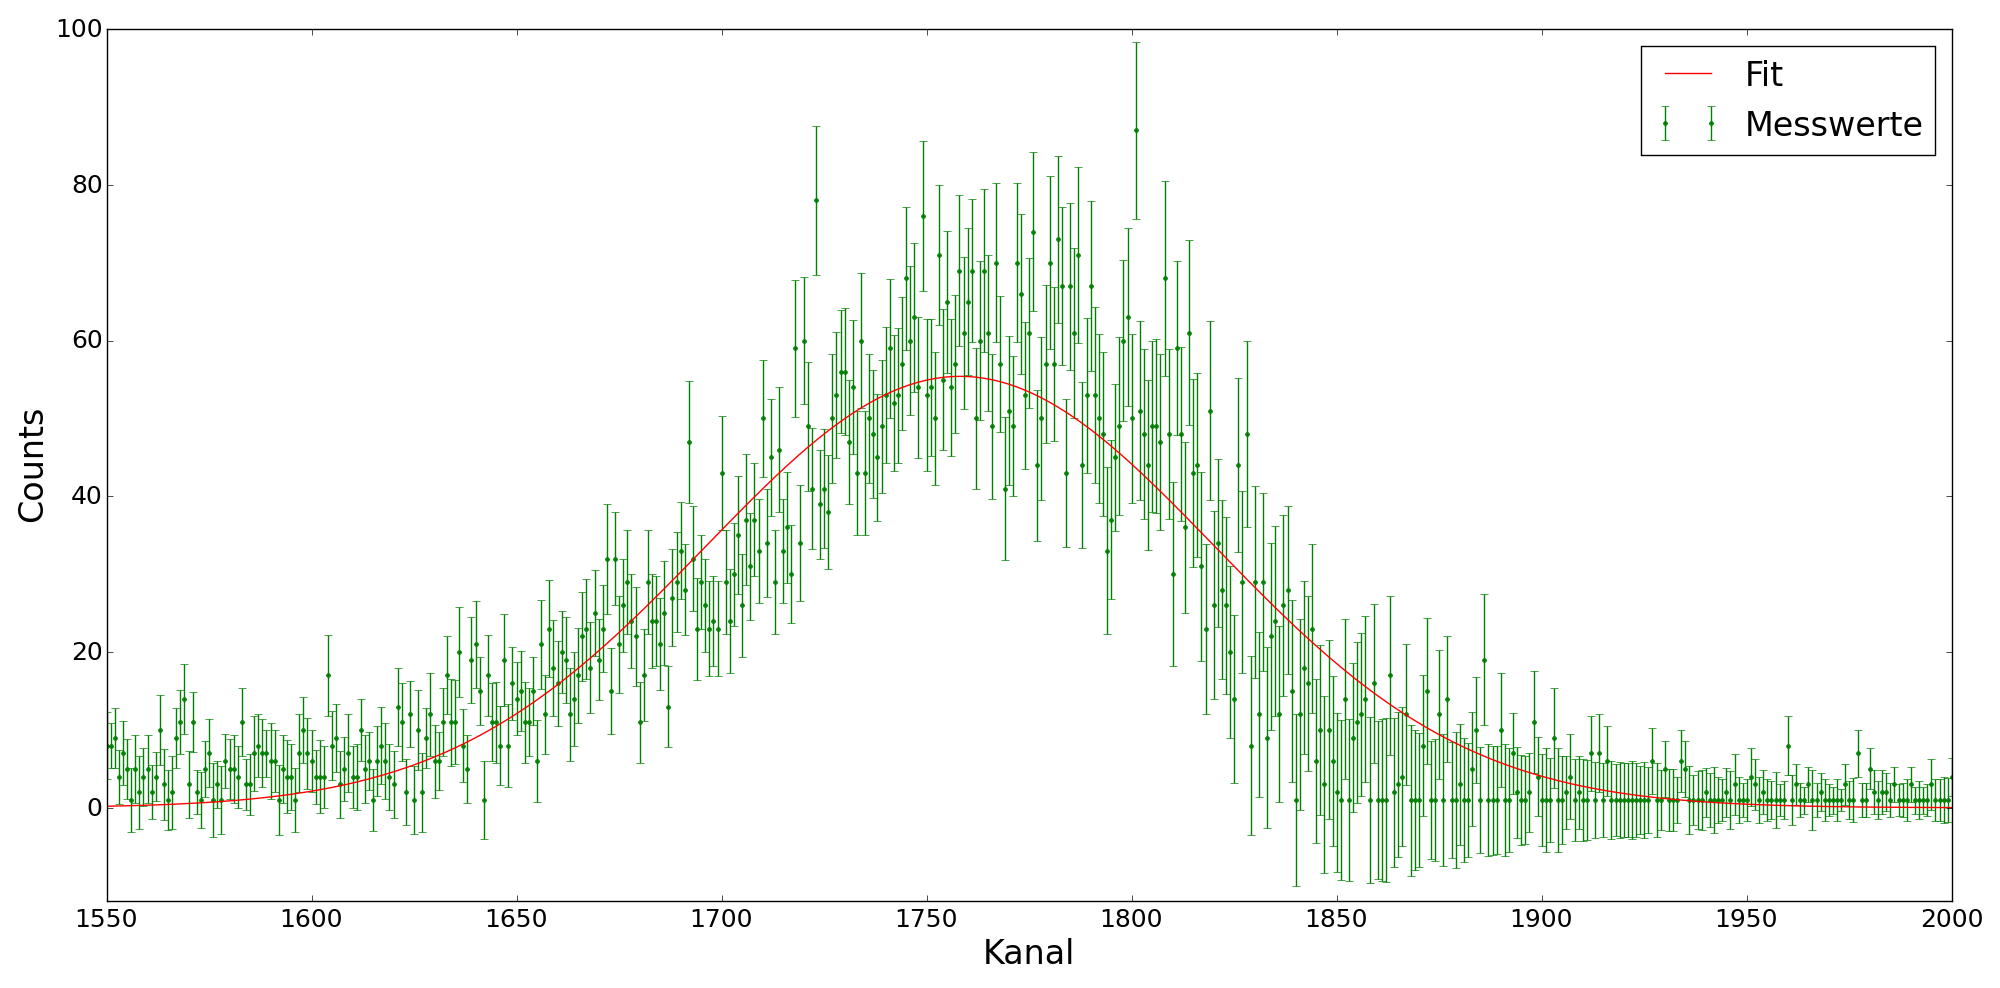
\includegraphics[scale = 0.34]{Wirkungsquerschnitt_30_Grad_Fit.png}
\caption{Die Fitparameter sind in Tabelle \ref{tab:30_Grad_WQ} eingetragen.}
\label{fig:Wirkungsquerschnitt_30}
\end{figure}

\begin{table}[H]
\centering
\caption{Fitparameter f�r die Energiemessung bei \SI{30}{\degree}. Das $\chi^2_{red}$ ergab sich mit 1.136}
\label{tab:30_Grad_WQ}
\begin{tabular}{|c|c|c|}
\hline Gau�peak & Parameter & Wert \\ 
\hline 1 & Amplitude & 8089(143) \\ 
\hline  & Center & 1758(1) \\ 
\hline  & Sigma & 53,5(7) \\ 
\hline 
\end{tabular} 
\end{table}

\begin{figure}[H]
\centering
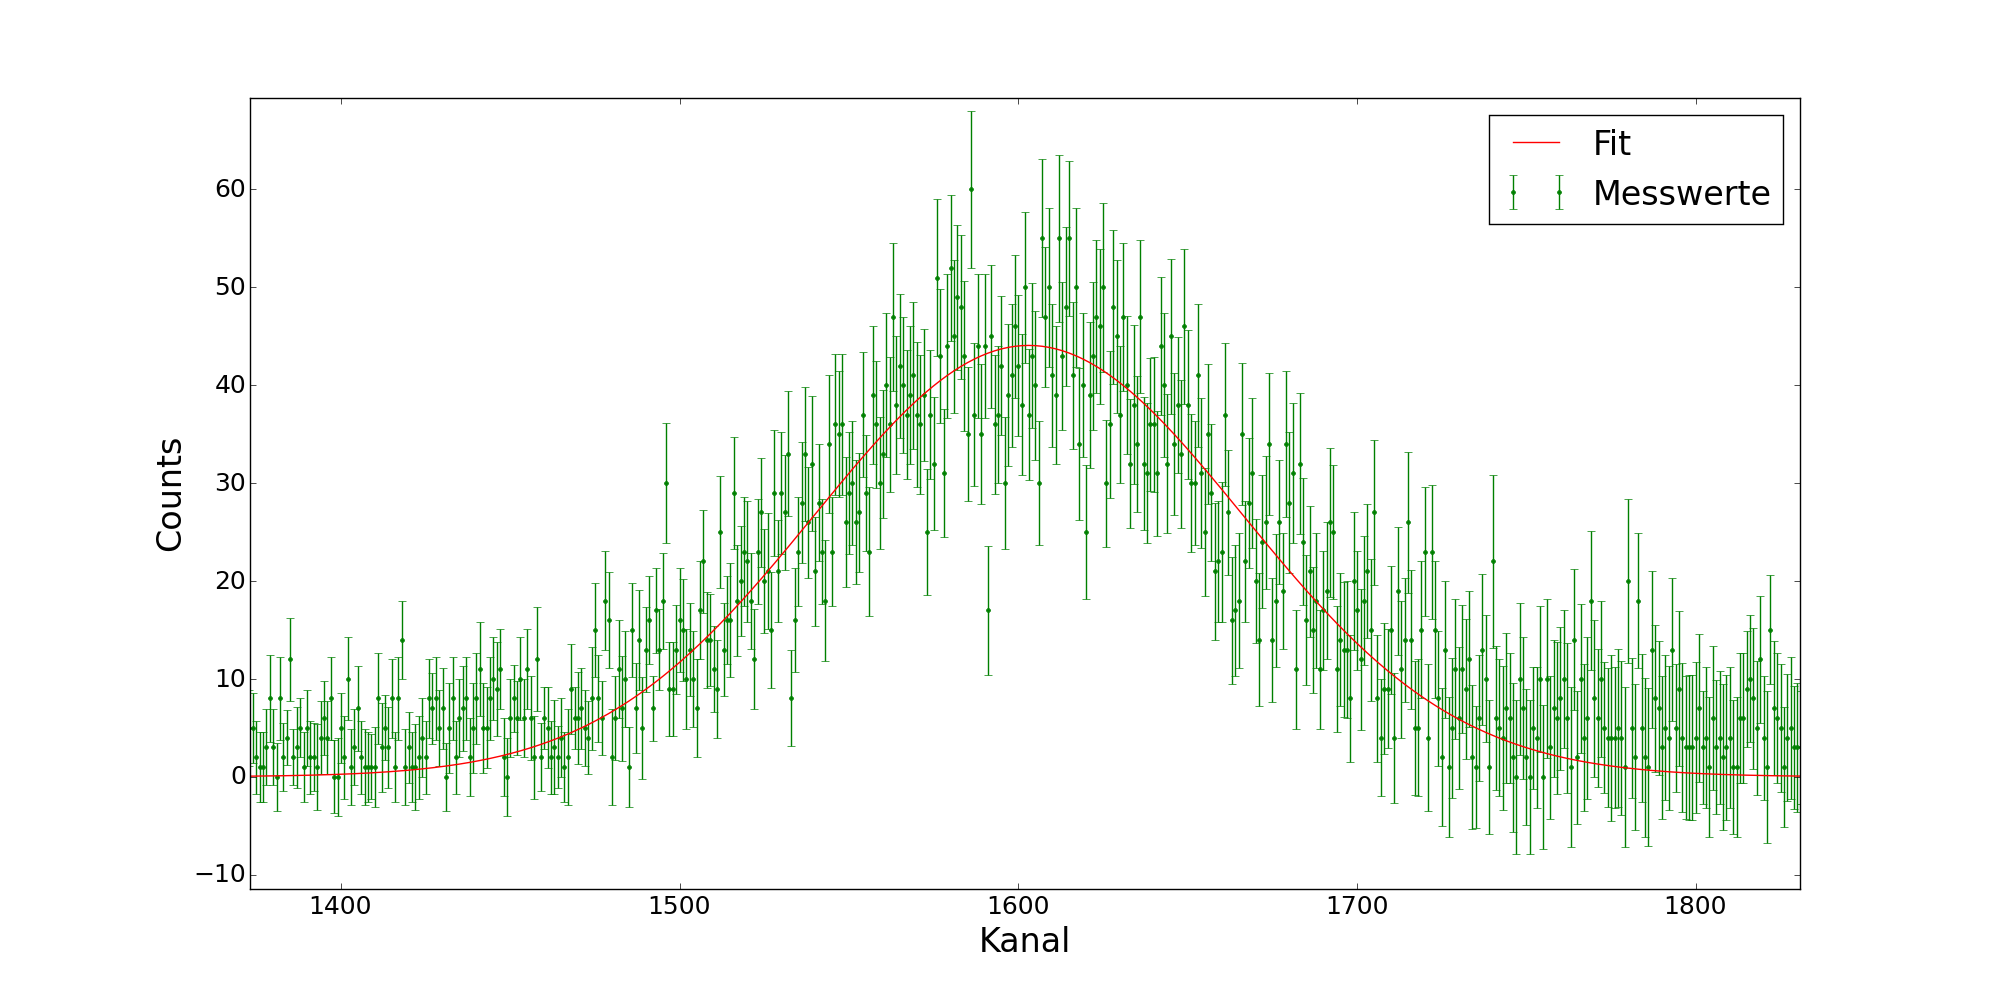
\includegraphics[scale = 0.34]{Wirkungsquerschnitt_40_Grad_Fit.png}
\caption{Die Fitparameter sind in Tabelle \ref{tab:40_Grad_WQ} eingetragen.}
\label{fig:Wirkungsquerschnitt_40}
\end{figure}

\begin{table}[H]
\centering
\caption{Fitparameter f�r die Energiemessung bei \SI{40}{\degree}. Das $\chi^2_{red}$ ergab sich mit 0.994}
\label{tab:40_Grad_WQ}
\begin{tabular}{|c|c|c|}
\hline Gau�peak & Parameter & Wert \\ 
\hline 1 & Amplitude & 6870(103) \\ 
\hline  & Center & 1602(1) \\ 
\hline  & Sigma & 63(1) \\ 
\hline 
\end{tabular} 
\end{table}

\begin{figure}[H]
\centering
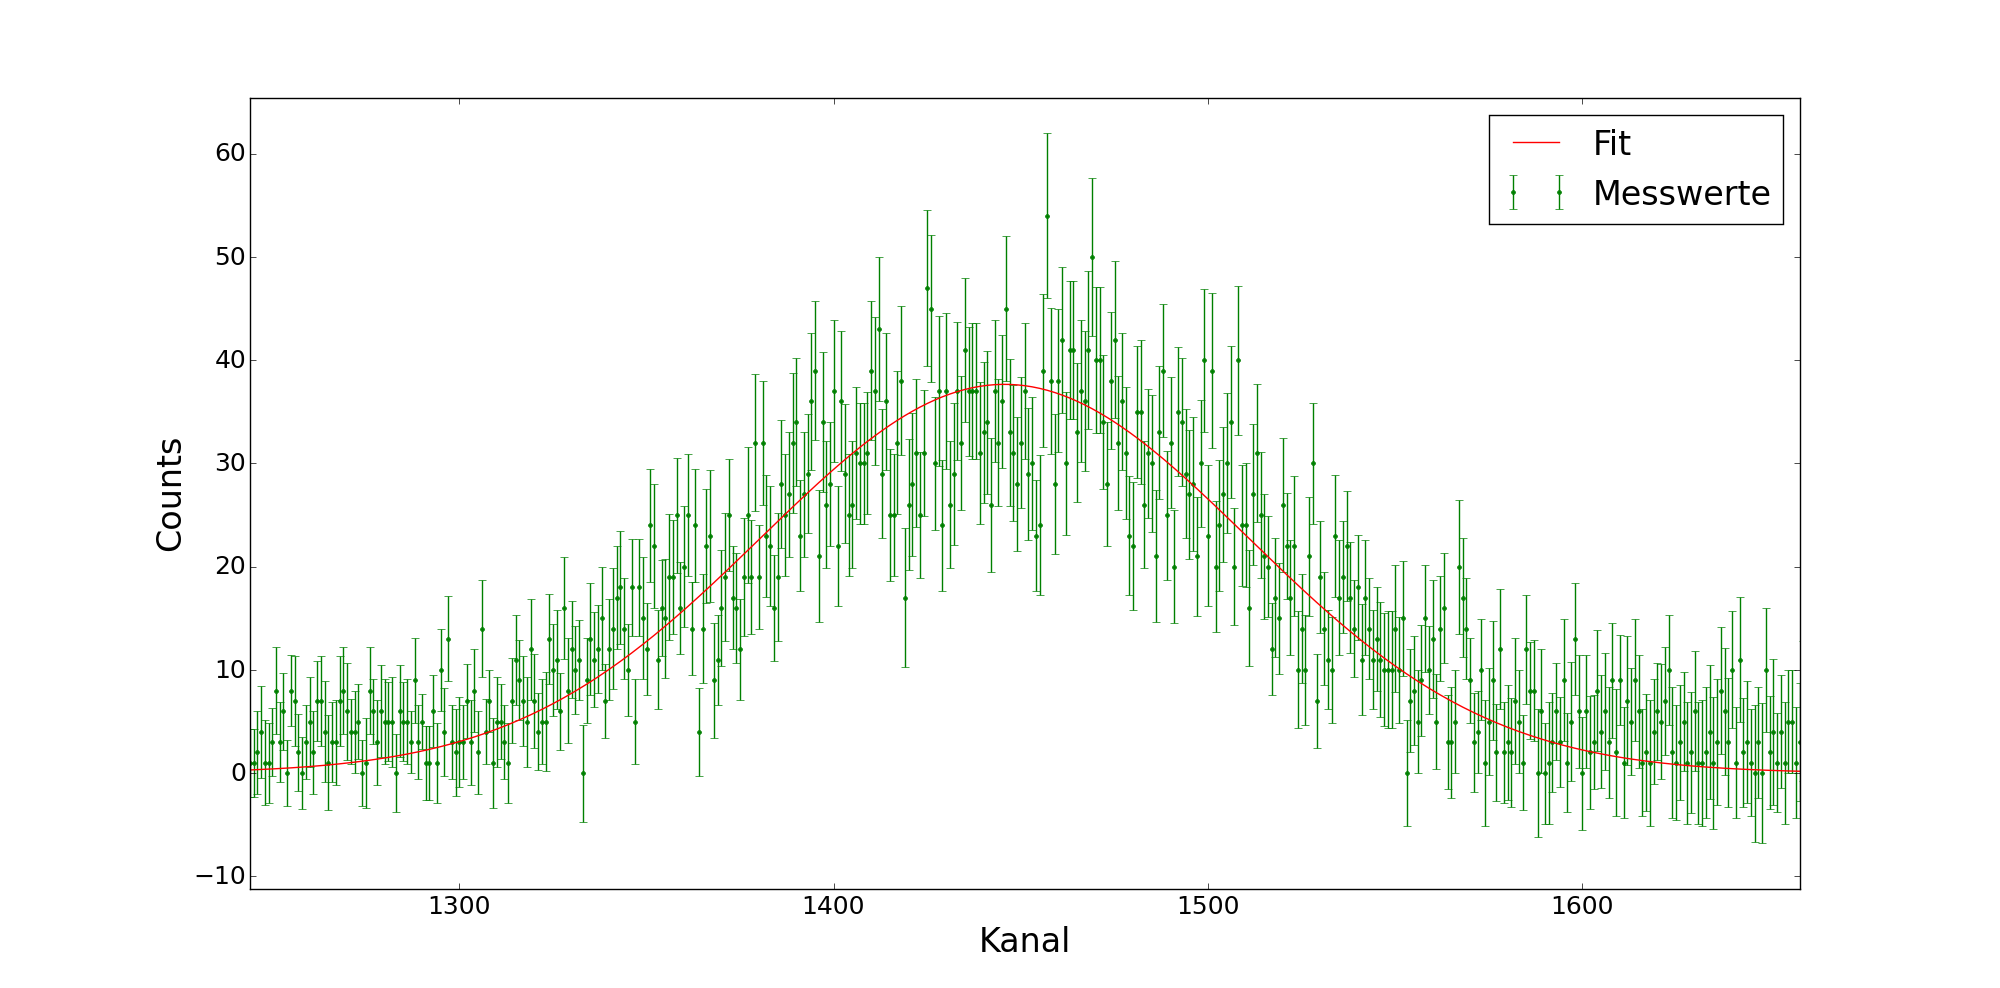
\includegraphics[scale = 0.34]{Wirkungsquerschnitt_50_Grad_Fit.png}
\caption{Die Fitparameter sind in Tabelle \ref{tab:50_Grad_WQ} eingetragen.}
\label{fig:Wirkungsquerschnitt_50}
\end{figure}

\begin{table}[H]
\centering
\caption{Fitparameter f�r die Energiemessung bei \SI{50}{\degree}. Das $\chi^2_{red}$ ergab sich mit 0.971}
\label{tab:50_Grad_WQ}
\begin{tabular}{|c|c|c|}
\hline Gau�peak & Parameter & Wert \\ 
\hline 1 & Amplitude & 5897(93) \\ 
\hline  & Center & 1445(1) \\ 
\hline  & Sigma & 63(1) \\ 
\hline 
\end{tabular} 
\end{table}

\begin{figure}[H]
\centering
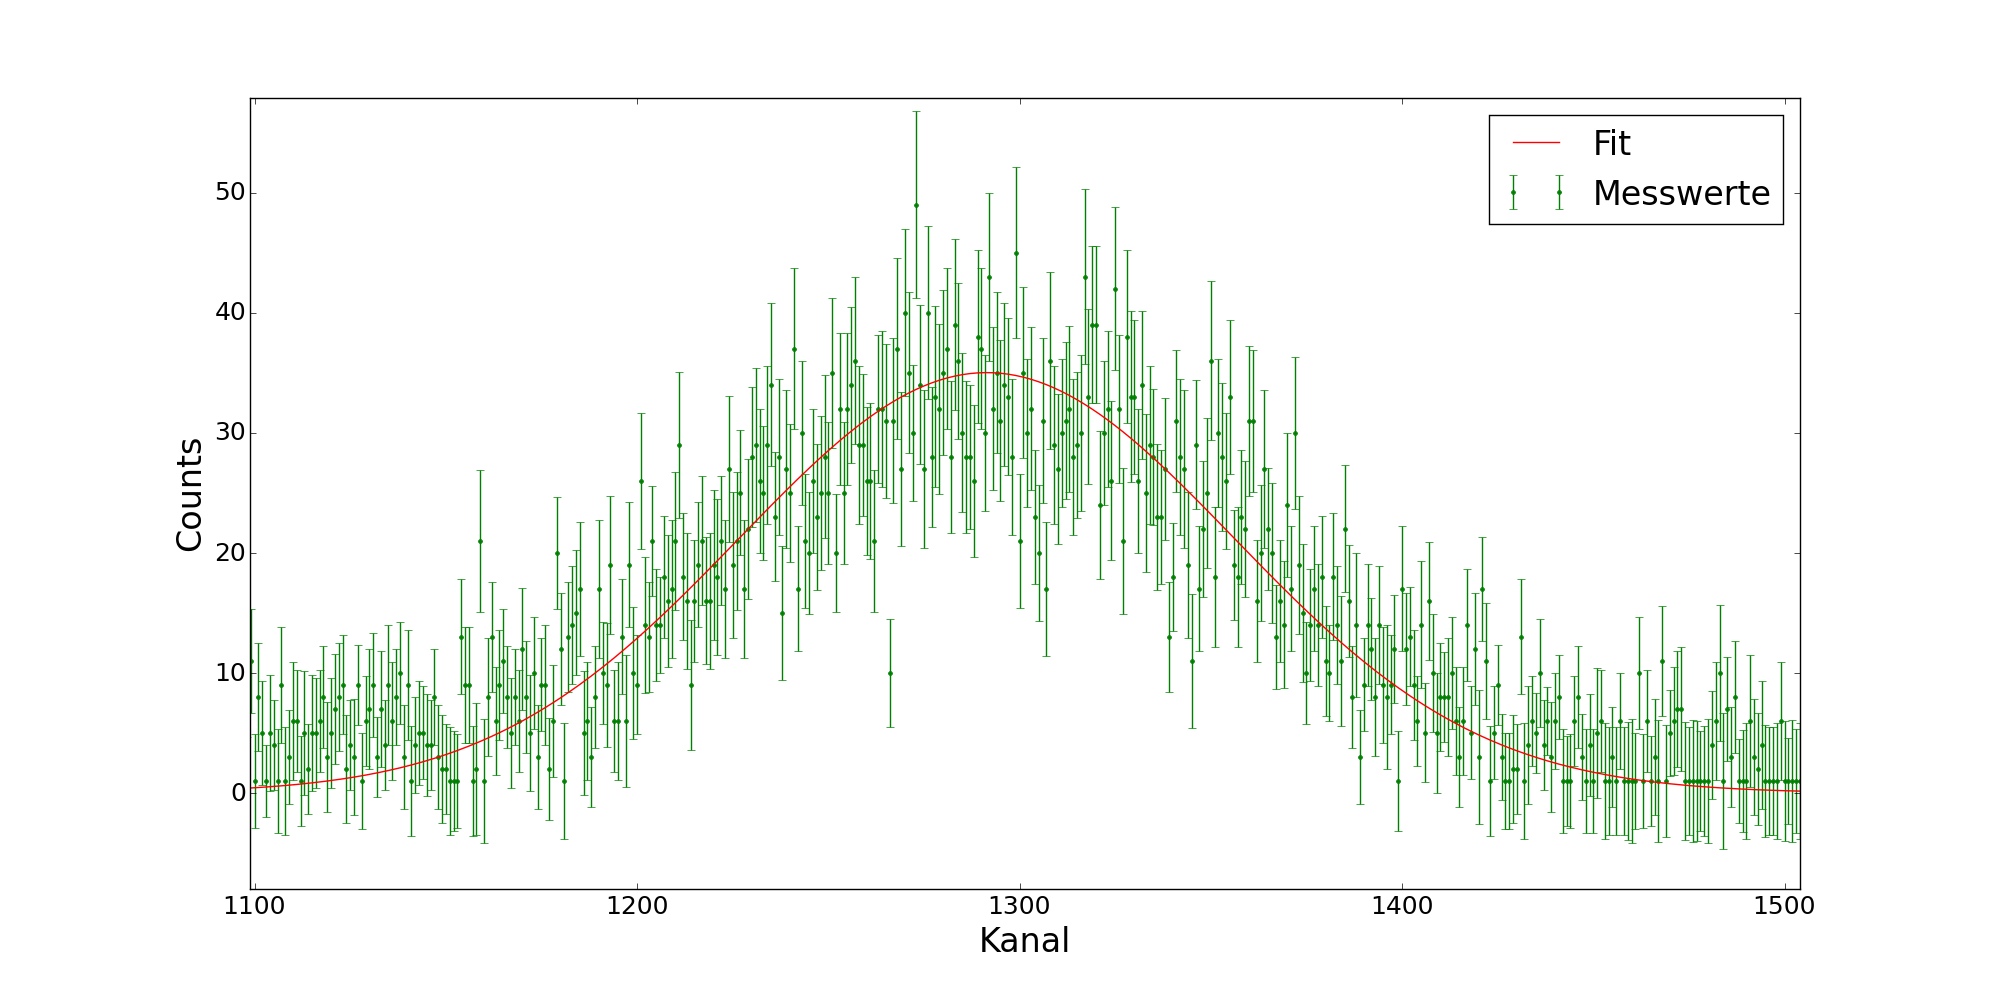
\includegraphics[scale = 0.34]{Wirkungsquerschnitt_60_Grad_Fit.png}
\caption{Die Fitparameter sind in Tabelle \ref{tab:60_Grad_WQ} eingetragen.}
\label{fig:Wirkungsquerschnitt_60}
\end{figure}

\begin{table}[H]
\centering
\caption{Fitparameter f�r die Energiemessung bei \SI{60}{\degree}. Das $\chi^2_{red}$ ergab sich mit 1.062}
\label{tab:60_Grad_WQ}
\begin{tabular}{|c|c|c|}
\hline Gau�peak & Parameter & Wert \\ 
\hline 1 & Amplitude & 5432(93) \\ 
\hline  & Center & 1291(1) \\ 
\hline  & Sigma & 63(1) \\ 
\hline 
\end{tabular} 
\end{table}

\begin{figure}[H]
\centering
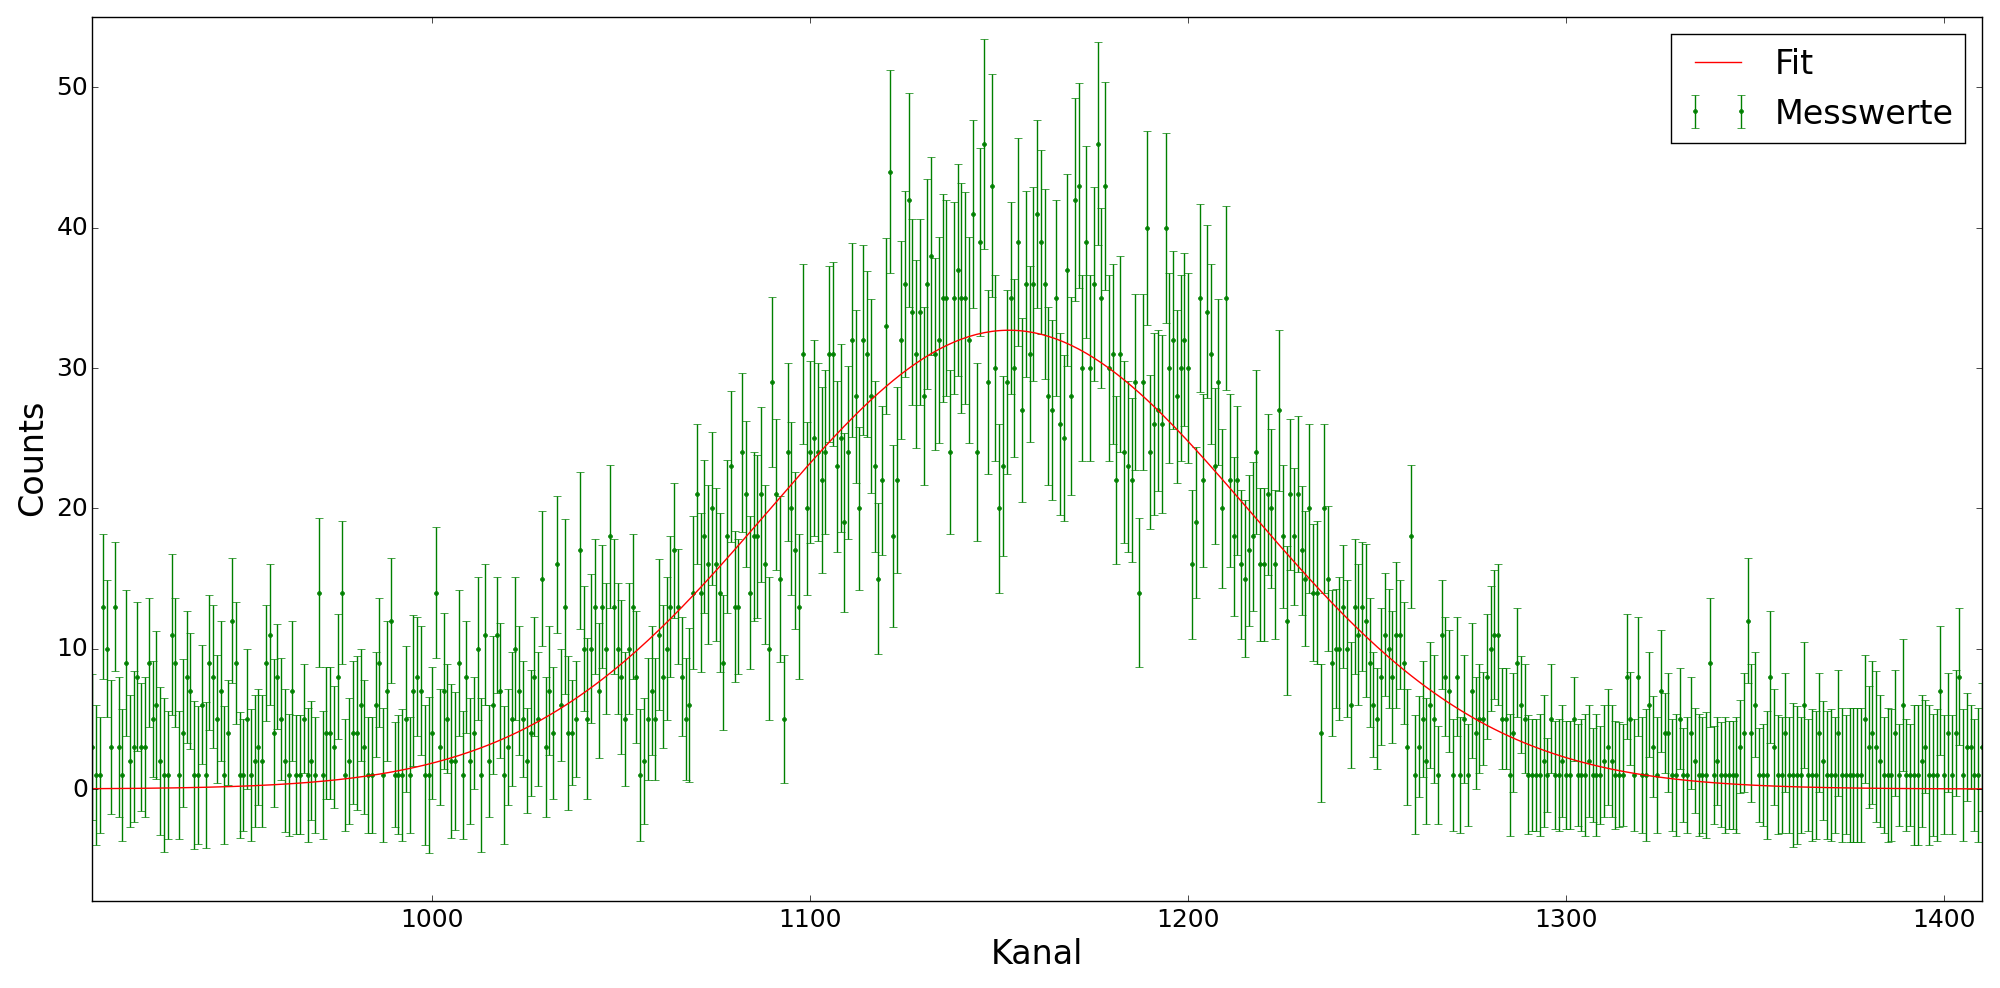
\includegraphics[scale = 0.34]{Wirkungsquerschnitt_70_Grad_Fit.png}
\caption{Die Fitparameter sind in Tabelle \ref{tab:70_Grad_WQ} eingetragen.}
\label{fig:Wirkungsquerschnitt_70}
\end{figure}

\begin{table}[H]
\centering
\caption{Fitparameter f�r die Energiemessung bei \SI{70}{\degree}. Das $\chi^2_{red}$ ergab sich mit 0.933}
\label{tab:70_Grad_WQ}
\begin{tabular}{|c|c|c|}
\hline Gau�peak & Parameter & Wert \\ 
\hline 1 & Amplitude & 5217(94) \\ 
\hline  & Center & 1152(1) \\ 
\hline  & Sigma & 64.0(7) \\ 
\hline 
\end{tabular} 
\end{table}

\begin{figure}[H]
\centering
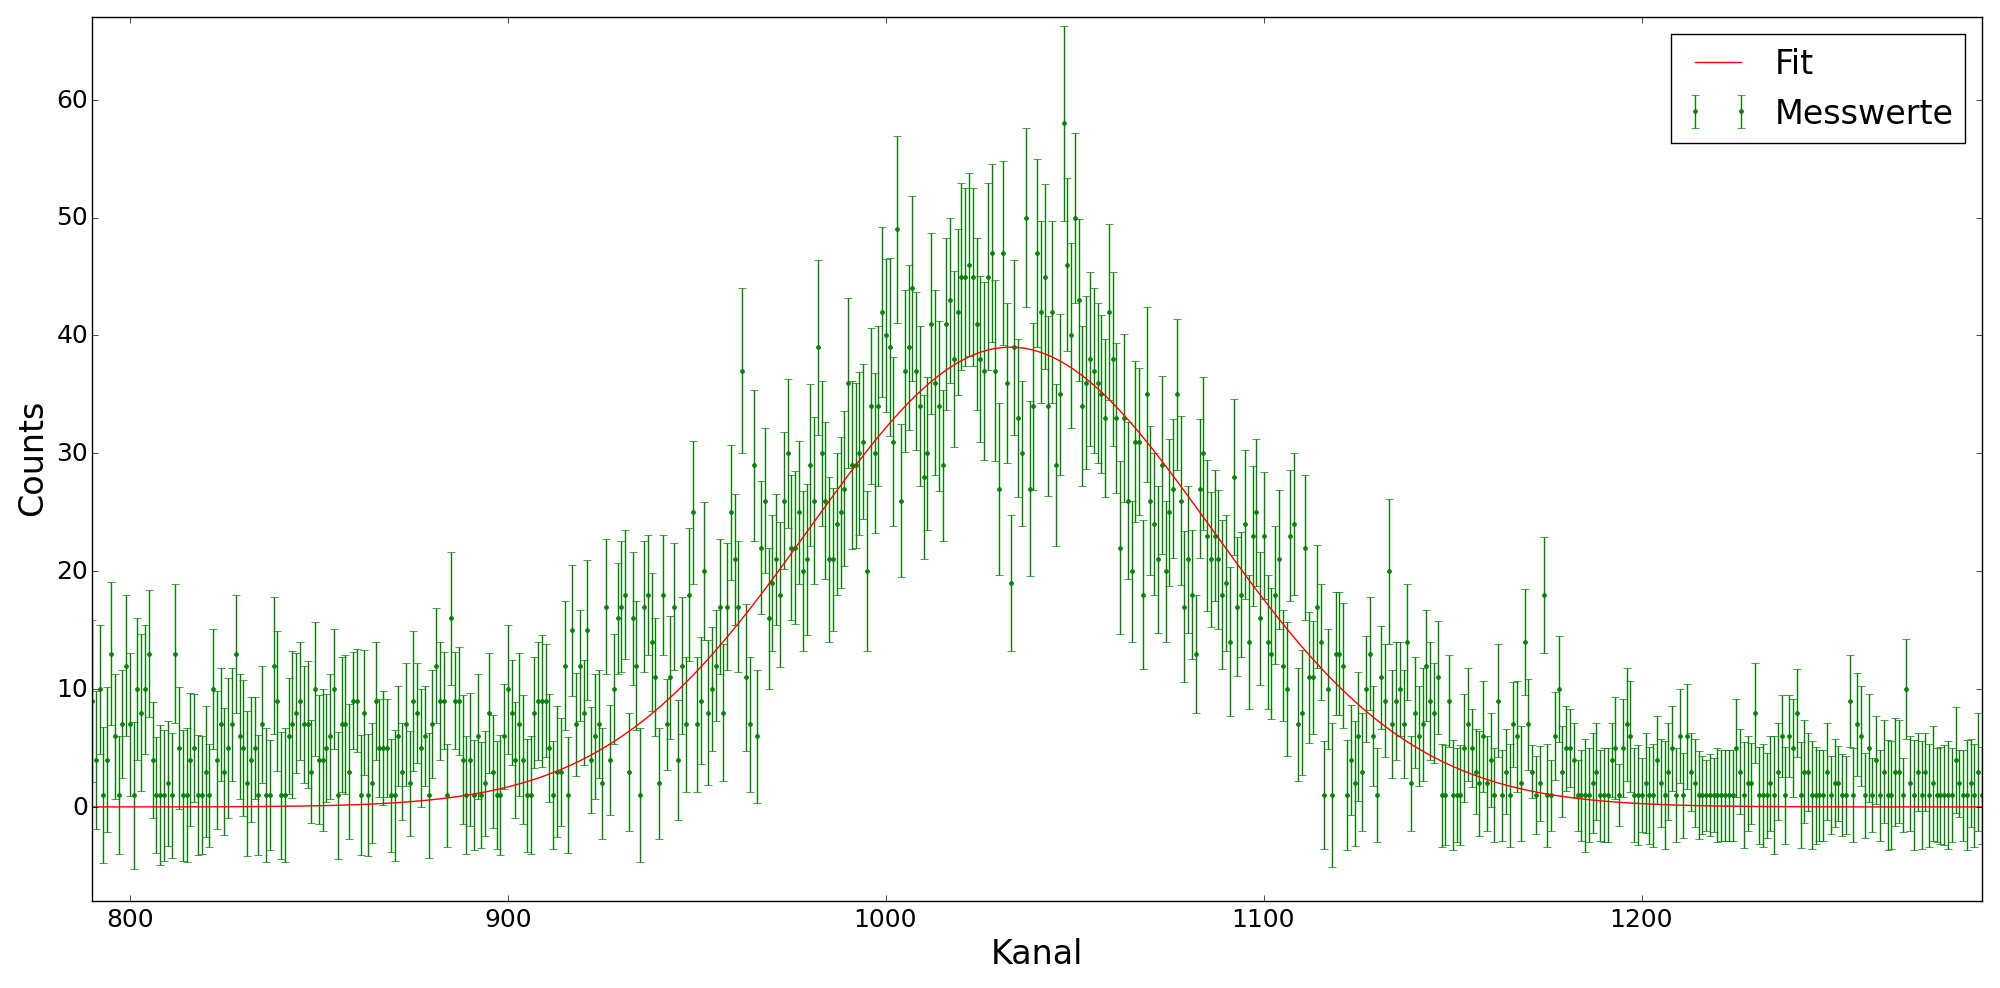
\includegraphics[scale = 0.34]{Wirkungsquerschnitt_80_Grad_Fit.png}
\caption{Die Fitparameter sind in Tabelle \ref{tab:80_Grad_WQ} eingetragen.}
\label{fig:Wirkungsquerschnitt_80}
\end{figure}

\begin{table}[H]
\centering
\caption{Fitparameter f�r die Energiemessung bei \SI{80}{\degree}. Das $\chi^2_{red}$ ergab sich mit 1.100}
\label{tab:80_Grad_WQ}
\begin{tabular}{|c|c|c|}
\hline Gau�peak & Parameter & Wert \\ 
\hline 1 & Amplitude & 5194(99) \\ 
\hline  & Center & 1033,0(8) \\ 
\hline  & Sigma & 53,1(8) \\ 
\hline 
\end{tabular} 
\end{table}